% !Mode:: "TeX:UTF-8"   %%winedt 以utf8编码打开
% Can only be compiled with xelatex+bibtex

%双行标题
\documentclass[twoside,longtitle]{LZUthesis}
%单行标题
%\documentclass[twoside]{LZUthesis}

\usepackage{float}
\usepackage{fancybox}
\usepackage{calc}
\usepackage{mathdots}
\usepackage{graphicx}
\usepackage{listings}

%声明图片后缀名
\DeclareGraphicsExtensions{.pdf,.eps}

\makeatletter

% 设置图形文件的搜索路径
\graphicspath{{figures/}}

% 小节标题靠左对齐
\CTEXsetup[format+={\flushleft}]{section}

% 取消链接的颜色(黑白打印时启用)
%\hypersetup{colorlinks=false}

%使文档居中,打印时应注释掉
\evensidemargin 0.93 true cm
\setlength{\hoffset}{-0.3 cm}

%允许equationarray分页换行
\allowdisplaybreaks

%使字体清晰,且透明位图不会使页面文字粗细不一
\usepackage{eso-pic}
\AddToShipoutPicture{%
\special{pdf: put @thispage <</Group << /S /Transparency /I true /CS /DeviceRGB>> >>}%
}

%页面背景色
%\definecolor{yellow}{rgb}{0.99,0.99,0.70}
%\pagecolor{yellow}

%浮动项超链接正确跳转
\usepackage[all]{hypcap}

\makeatother


\begin{document}

%分类号;一般不要求学生填写
\classification{}

%密级;申请保密后需填写
\confidential{}

%中文标题
\title{机器学习技术分析与有效市场实证研究}

%中文标题第二行,题目较短时删除之,并去除文档类选项 longtitle
% \titleadd{\LaTeX{}模板简介}

%英文标题
\englishtitle{Introduction to the \LaTeX{} Template of}

%英文题目第二行,题目较短时删除之,并去除文档类选项 longtitle
\englishtitleadd{Lanzhou University Thesis}

%作者汉语姓名
\author{孙力骏}

%专业
\major{应用统计}

%学位
\degree{硕士}

%研究方向
\direction{机器学习}

%导师姓名+职称
\advisor{李周平~教授}

%论文工作起止年月
\datebeginAndEnd{2019年10月至2021年4月}

%论文提交日期
\submitdate{}

%答辩日期
\defenddate{}

%学位授予日期
\degreedate{}

%左侧页眉
\lzuthesis{兰州大学硕士学位论文}

%生成封面
\maketitle

%生成声明页
\makestatement

%前文-罗马页码
\frontmatter\pagenumbering{Roman}

%中文摘要
\begin{abstract}
本文是兰州大学学位论文的\LaTeX{}。(包含LyX)模板及其使用说明。除了介绍文档类LZUthesis的用法外,本文还是一份简要的学位论文写作指南。
\end{abstract}

%中文关键词
\keywords{兰州大学,学位论文,\LaTeX{}模板,LyX模板}

%英文摘要
\begin{englishabstract}
This paper is a \LaTeX{} (include LyX) thesis template of Lanzhou University. Besides the usage of the LaTeX document class LZUthesis, a brief guideline for writing the thesis is also included.
\end{englishabstract}

%英文关键词
\englishkeywords{Lanzhou University, Thesis, \LaTeX{} Template, LyX Template}

%自动生成章节目录以及pdf书签
\tableofcontents{}

%正文部分-数字页码
\mainmatter

%正文页眉页脚样式
\pagestyle{lzu}


\chapter{绪论}

\section{研究背景}
金融市场\cite{hesengming1990}是由一系列不同的以金融工具作为交易对象的市场组成的一个庞大的体系,是交易金融工具的场所。其结构复杂,种类繁多,包含但不限于票据贴现市场、短期存贷款市场、国库券市场、同业拆借市场、长期贷款市场、股票市场、外汇市场、贵金属市场、标准化的商品市场和衍生品市场等。金融市场的健康发展对于国民经济而言是至关重要的,一般认为,金融市场具备以下四大功能\cite{mishkin2007}\cite{zhangyichun2002}:
\begin{enumerate}
    \item 金融市场可作为资金融通的通道和媒介
    \item 金融市场的交易行为所产生的价格可作为衡量经济的标尺
    \item 为管理部门的宏观调控提供介质
    \item 提供了风险分散与转移的工具
\end{enumerate}

从资金融通的角度来看,金融市场可快速引导资金合理流动。如此,资金会从盈余方流向赤字方,从相对收益率较低的经济机会流向相对收益率较高的经济机会。金融市场使得投资者的资金有了去向,而资金的需求者,也可支付一定报酬作为成本,获取资金的使用权。以此,提高了资金配置的效率,进而提高经济发展的效率和全要素生产率。

从价值标尺的角度来看,金融市场具备价值发现功能。不论是企业资产,还是大宗商品或农产品,亦或是贵金属,金融市场常常决定了这些产品的价格。如果这个价格与企业的内在价值接近或相同,那么,好公司或好产品就能获得更多的资金支持,从而使得经济向健康的方向发展。反之,如果金融市场的定价不准了,质地优良的公司及其优秀的管理层和员工,则可能难以得到足够的社会资源的分配,导致资源的利用效率下降,进而影响全要素增长率的提高,最终影响到国民的获得感和幸福感。

金融市场的价值发现功能对于国民经济的稳定运行和良好发展发挥着至关重要的作用,本文也将从全新的角度,详细地研究这个问题。

从管理部门进行宏观调控的角度来看,金融市场是良好的政策性工具的施展处。例如,中国人民银行可在银行间拆借市场进行公开市场操作,也可以在境外的离岸人民币交易市场发行或回购央票,美国联邦储备银行则通过联邦基金市场的利率来影响美国经济,乃至于量化宽松(quantitative easing),甚至为了应对covid-2019疫情,美联储还会买入公司债券以稳定市场。如果没有金融市场的存在,经济管理当局的政策将难以有效得到贯彻。而实际上,管理当局进行的宏观调控也需要良好的价值发现功能作为支撑,否则,政府救市或调控,则难以把资源投入优秀的公司,不利于经济生态。

金融市场还可实现风险的分散和转移,这与投资者进行控制风险(risk)和回报(return)的微观决策和管理提供了帮助。对于每个经济人而言,持续经营与稳定发展都离不开金融市场。以通过支付宝渠道进行销售的天鸿货币基金(又称余额宝)为例,消费者可以只需购买这个货币基金,就可实现远高于活期存款的年化收益率,以及匹配现金的流动性。而对应标的物形成的风险,依据中心极限定理(CLT)则可能由于相互独立而被抵消掉。

从以上对于金融市场功能的分析来看,金融市场良好与健康的发展,需要充分发挥其价值发现功能。在各级金融市场,尤其是资本市场上,需要建立与培养健康的经济生态。资本市场价格这个“经济晴雨表”,需要贴切地反映上市公司的经营质量和管理层的管理能力、职业道德以及公司的社会价值。

没有良好的价值发现功能,资本市场也就很难吸引各类投资主体的参与,同样地,也很难吸引优秀的企业前来发行各类金融工具。没有良好的价值发现功能,市场就难以累积足够的人气,宏观调控与风险转移的功能也就难以实现。鉴于金融市场价值发现体制机制的重要性,本文将着眼于有效市场假说与金融市场价值发现功能的研究上。

\section{我国金融市场价值发现功能发展简史}
本节将从价值发现的角度来谈中国金融市场的发展\cite{zhouxiaochuan2010}。

新中国成立后,人民政府没收了官僚资本主义的银行,并对金融业进行了社会主义改造。在此基础上建立起高度集中统一的国家银行体系。50年代到70年代,中国金融业具有“大一统”的显著特点,高度集中的“大一统”国家银行体系与众多的农村信用合作社相结合是50~70年代中国金融业的最显著特点。

改革开放以来,中国的金融业从“大一统”走向了金融自由化。上海证券交易所、深圳证券交易所以及商品期货、金融期货、黄金、外汇等交易所蓬勃发展,带来了金融市场的空前繁荣。其中,利率曾经长期严格管制,银行体系商业竞争力低下,缺乏活力。同时,资本市场被过度管制,寻租现象时有发生。商品市场交易规则不规范,一系列重大事件体现出金融市场价值发现功能的不完善。

其中,期货市场触目惊心的大型多空对垒就发生了至少几十次。上海327国债期货事件,出现数家机构联手操纵市场,造成交割日当日价格走势大幅波动。尤其是1995年2月23日,空方主力进行大额裸卖,将当日开仓的多头全数打爆,使得327合约暴跌了38元。之后,证监会暂停了国债期货的交易试点,中国第一个金融期货产品夭折,直到十几年后才恢复。

股票市场方面,早期的中国股市的价格发现功能也较为疲软。优秀的公司未必会获得高额的市场估值,而一些热衷于概念炒作,由一些江湖团队进行运作的小公司,却往往走出大行情。在2000年底到2001年初,“庄家”吕梁与深圳某大户勾结上市公司管理层,将一家名叫康达尔的,以养鸡为主营业务的上市公司,包装改造成了“科技+”概念股票,并将公司名称改名为“中科创业”。通过运用资金“坐庄”,将股价建立在了完全的虚无之上。也就是,一方面,吕梁勾结上司公司管理层,操控管理层的消息源;另一方面,吕梁及其手下的多位活跃在各个证券营业部的融资、操盘大员,通过对敲等技术手段,伪造交易数据。在吕梁的操纵下,中科创业的股价一路飙升。1999年7月,中科创业的股价从之前的36元跃升到了45元,到了2000年2月,中科创业的股价上升到了80元。

从今天回望,如果中科创业的操纵市场的团伙不发生内部矛盾,如果那位来自深圳的大户不提前斩仓获利出局,这位“神庄”可能就会在高位成功套现,广大中小投资者最终将蒙受巨量损失,从而对股票市场心灰意冷。

进入二十一世纪之后,中国金融市场走向了更加市场化和规范化的道路。诸如,327国债事件、中科创业操纵市场案、蓝田股份财务造假案以及银广厦财务造假案,这类耸人听闻的现象已经变得越来越少。中小投资者与机构投资者在市场中的占比也在悄然发生变化,国内外基金经理的素质明显提升,相关的财务审计标准,以及交易细则的完善,也有利于金融市场价值发现功能的稳步实现。但是,2013年,中国股市出现了“钱荒”事件,之后的2015年,中国股市发生股灾,场外配资平台的问题浮出水面,“穿仓”或“爆仓”现象层出不穷。

因为,我国金融市场价值发现功能是在不断发展和前进的,因此,本文着眼于近3年的深圳市场,从数据出发,进行中国股市的价值发现功能状况的实证研究,最终使用,使用机器学习的思想和方法来论证我的观点。

对于价值发现功能的评价,可通过市场有效性\cite{Malkiel1970EFFICIENT}来获得。市场有效性有可简单分为弱式有效(weak form)、半强式有效(semi-strong form)和强有效(strong form),本文将重点探讨弱有效性相关问题。

\section{本文研究的内涵与意义}

本文将从价值发现这样一个对金融市场而言极其重要的功能入手,探索市场价格是否已包含了市场数据信息。结合统计机器学习、贝叶斯优化和因果推断等方法,提出一套全新的论证市场弱有效性(weak form)的测试体系和判断逻辑,并最终判定我国股票市场的弱有效性。

与弱有效性相关的,是技术分析能否盈利的问题。我国股票市场中,中小投资者往往信赖技术分析,并在技术分析各种指标体系上投入了大量的时间和精力,以期待通过技术分析从市场中获得超额利润。本文则有力回答了技术分析到底能否从市场中盈利这个问题。

本文以机器学习的视角来理解金融市场,对我国股票市场的弱有效性进行了论证,其不失为之前学说的补充。本文结尾还将综合本文的实验结果,提出一些政策性的建议,讨论金融市场有效性需要哪些政策支持。

\section{本文结构}
本文将按如下结构来书写。
\begin{itemize}
    \item 第一章是导言,阐述中国市场的定价问题,以及概述本文的内涵与意义。
    \item 第二章介绍本文的背景知识与文献综述,包括,股市交易的基本分析知识和技术分析知识、机器学习、深度学习、因果推断。包括有效市场假说以及有效市场假说在中国股市和其他市场中的实证研究。
    \item 第三章从理论上阐述本文所使用的方法,提出了贝叶斯优化技术分析这样一个交易体系。
    \item 第四章是实证分析与细节。
    \item 第五章是结论与未来展望。
\end{itemize}


%---------------- Chapter 2 ---------------------------
\chapter{背景知识与文献综述}
\section{股票及股票市场}
\subsection{概述}
股票(stock)\cite{xiaoyimin1996} 是股份公司发行的所有权凭证,股票持有者享有从股票发行的股份公司取得股息,以及在公司的最高权力机构——股东大会上投票的权力。股票也是一种金融工具,是资本市场上主要的长期信用工具,对标的公司享有剩余价值,但不得要求发行公司返还出资。
股票市场就是用来买卖股票的场所。股票市场分为交易所和场外交易两大类。我国目前存在上交所和深交所两大交易所,同时也有三板市场,创投市场等多种买卖股票的场所。一般认为,股票市场分为发行市场和交易市场。
发行市场常常被称为一级市场,一般来说,是指股票首次公开发行(initial public offering)时,股民或机构的认购交易,属于一级市场的交易。一级市场的交易,常常由投资银行或证券经纪人予以承销或分销,在我国,上市公司IPO发行的股票,常常以略低于市场价值的价位确立为中签价。随后,投资者可根据存量股持有量和投资资金量及其他规则,来确定中签几率,最后,凭借随机抽签的结果,来确定股票的最终出售对象。
二级市场则是指已发行的有价证券买卖流通的场所,是转让有价证券的地方。我国的深交所、上交所设有多个二级市场交易版块,交投活跃。日交易量平均达到5500亿人民币作用。二级市场的存在,为股票的持有者提供了充足的流动性。同时,二级市场的定价功能的优劣,也成为了一级市场发展,乃至相当程度的实体经济发展的一个根本指针。本文将从机器学习的视角出发,详细研究股票市场的价值发现功能,归根结蒂研究的对象是二级市场交易价与股票实际价值之间的关系问题,这个问题也可以被定义为股票市场有效性问题。

股票市场与实体经济关系密切,
一级市场常常被认为是股票市场的起点,但实际上,多数公司的起点并不是一级市场。一个创业公司,常常是由创业合伙人投资组成。合伙人自掏腰包,或从家人、亲戚、朋友处筹集资金,是为种子轮。之后拿到的第一笔融资,常常被称为天使轮。天使轮往往是大型资本的富有远见的运作,这部分资金承担了创业的高风险,如果创业失败,这批资金将遭受损失,不过,承担高风险的同时也会享受创业成功后的高收益。如果创业成功,天使轮的投资将获得极高倍率的回报。种子轮以及天使轮之后,初创公司往往还要经历多轮融资,每一轮的融资金额次第上升,而投资者的最终的回报也会逐渐降低,但风险也会相应下降。最终,初创公司的部分团队,以及为初创公司提供帮助和弹药的创业投资资本,将需要一个提供合理报价和估值的股权交易市场来退出,为他们对社会做出的贡献索取合理的报酬。初创公司各方的退出通道,往往需要公司进行首次公开发行,因此,一个成熟、价值发现功能完备的股票市场,对于一个国家或经济体系的发展来说,常常是不可或缺的。



天使轮企业需要有详尽的创业计划和业务计划。而对天使轮进行投资,需要专业机构进行《尽职调查报告》(due diligence report),也称DD。经过种子轮的投资,一家企业可能从萌芽状态开始生长,而专业机构将对一大批萌芽企业进行遴选,以专业的视角支持或拒绝一大批企业。优秀的企业将继续存活,而资质欠缺的企业,或许以小企业的身份固守一个较低的生态位,也可能被市场所淘汰。

从机器学习的视角来看,天使轮常常意味着专业投资机构对企业信息的第一轮挖掘。描述了一种数据分析模型,这种模型可以让风险投资基金更好地把握早期初创公司的价值,以做出更加正确的投资。Wu解释了中国和美国在科技创业公司方面的差异问题。他提出的这项数据驱动型的判断模型显示出了良好的效果。

但风险投资者与创业者的关系,有时又往往是双向的。创业者常常会得到风险投资者不限于资金支持的帮助。风险投资资本常常会派遣人力前往支援,或提供一些物力上的帮助。因此,风险投资者除了对创业者进行了数据挖掘,筛选出了优秀的创业者并支持他们的发展,同时淘汰了不够有利于社会经济发展的创业者,还可能深度参与经营活动,为创业者提供指导,增强了新兴的经济活动的活力。

我国的多种经济成分内,有相当数量的大型企业,是由上文所述的方式予以孵化、成长的。遗憾地是,截止到本文撰写,大量的国内新兴高科技或互联网企业所以来的股票市场是美国纳斯达克股票交易所,或者香港联交所,而不是我国的深圳证券交易所或者上海证券交易所。从以上模式孵化而出较著名的企业有美团点评(联交所代码:03690)、京东(纳斯达克代码:JD)、阿里巴巴(纳斯达克交易代码:BABA)等等。随着瑞幸咖啡的财务造假事件发酵,中概股在美上市所产生的诸如VIE结构、审计程序等种种问题开始被关切,如果我国自身的股票市场的成熟度可以接纳这些优秀的公司,那么,也一定可以吸收和利用来自全世界的聪明的资金,从而一举解决中概股异地上市所产生的各种问题。本文研究中国股市的有效性,正是因为其对于我国经济发展是至关重要的。

我国内地还有多种不同性质的公司,通过多种途径上市。例如,地方国资委可以通过国有企业改制的方式,将一些明星资产打包整体上市,从而拥有上市公司平台,起到扩大市场规模和影响力,背书增信的积极作用。我国股市对于我国金融体系的稳定,规范金融公司的经营,提升效率,缓解金融抑制也做出了相当的贡献。限于篇幅,本文就不再一一分析。

总之,我国股市与我国经济的平稳较快健康的发展关系密切。

\section{基本分析与技术分析}
\subsection{基本分析}

基本分析(fundamental analysis)\cite{benjisming2009},也被称为基本面分析,是指投资者主要通过分析上市公司的盈利能力,估算其内在价值(intrinsic value)。基本分析派的投资者,常常根据这个内在价值来确立交易动作,以获得盈利。

基本分析中的内在价值,通常认为是未来股利的折现。$P$是现有的股票价格,$g$是一个常数股利增长率,$r$是一个常数代表企业的资本成本,$D_1$是下一年的分红(dividends):
\[
P=\frac{D_1}{r-g}.
\]

哥顿模型(Gordon model or Gordon's growth model)也可用来进行股指计算,该模型假设股利在未来以一个常数的增长率增长。哥顿模型\cite{hamada1969portfolio}的股价计算公式如下:
\[
P=\mathbf{D}\cdot\sum_{i=1}^{\infty}\left(\frac{1+g}{1+k}\right)^i=\mathbf{D}\cdot\frac{1+g}{k-g},
\]
这里,$P$是估计的股价,$\mathbf{D}$是最近一期每股的股利分配,$k$是折现率,$g$是股利未来的增长率。
这个折现股指模型,假设未来每年公司提供的股利(dividend)都是不变的,且未来的折现率也不变,因此,股价是股利除以折现率。

除了股利折现模型外,自由现金流折现模型(discounted cashflow model)也是投资领域广泛被采用的一个模型。该模型的计算方式如下:
\[
P=\sum_{i=1}^{\infty}\frac{\mathbb{E}[\mathbf{cf_i}]}{(1+r)^i},
\]
其中$cf_i$代表未来第$i$期对应的标的企业所产生的自由现金流。如果该企业为上市公司,则往往
\[
P\le\sum_{i=1}^{\infty}\frac{\mathbb{E}[\mathbf{cf_i}]}{(1+r)^i}.
\]
因为一家公司的未来现金流往往是不稳定的,对于不稳定的现金流,其回报率应该再加上一定的风险补偿。

那么,基本分析的目标就是准确地预测公司的未来盈利情况,对此,基本面分析常常包含了宏观分析、行业分析、公司分析等。宏观分析侧重于研究国家经济发展政策,以及以国家或区域经济(新兴市场、成熟市场、金砖四国等等)作为分析对象,判断一个经济体的健康状态和经济发展的阶段,从而进行宏观方向上的投资,和资产全球化的配置。行业分析则侧重于分析行业盛衰周期,行业技术的未来走向以及行业整体的发展状况。公司分析则分为很多种,最简单的就是业绩分析。投资者通过分析公开的财务报表数据,通过计算一些会计比率,阅读会计报表附注等方式,选择财务指标优秀的公司。这也是我国市场上最常见的“基本分析派”。因为我国金融体系的特殊性,我国的银行股常常以较高的杠杆率和较低的市盈率出现在股票市场之中,这些银行股业绩优良,市盈率低至4到5之间,吸引了大量此类“基本分析派”投资者的购买。

但以上基本面分析又不足以概括基本面分析的全貌。我国市场中,并购重组和高送转也是炒作热点。一些水平很高的股民,往往反而喜欢购买垃圾股。所谓垃圾股,就是主营业务开展不顺利,难以保持增长,甚至已然亏损,面临退市风险的股票。炒作垃圾股的逻辑很简单,因为,垃圾股的市值低至10亿,而由于我国的IPO发行制度非常严格,通过重组完成上市,可能存在政策套利的空间。根据估算,一个上市公司的壳价值超过30亿,由此产生了垃圾股玩家的盈利空间。

从传统思维方式很难全面理解基本分析,因为基本面分析相当于对世界上存在的所有信息进行挖掘,以寻找投资机会。例如,近期美国浑水基金做空瑞幸咖啡的报告中,他们派遣全职或兼职的员工上万人蹲守瑞幸咖啡店,通过视频取证,最终得出了瑞幸咖啡销售数据造假的结论。最终,在浑水公司的做空报告发出三个月后,瑞幸股价暴跌,通过衍生工具或合约做空该股的投资者获得了不菲的收益。

从机器学习的角度,则可很好的理解与解释基本面分析,以及基本面分析对于市场的作用。在机器学习(或称学习)的视角下,进行基本分析,实际上是一个数据挖掘的过程,或者更广义地说,是一个信息挖掘的过程。投资者通过对基本面信息进行分析和解读,形成了自身对于股票所代表的剩余权益的价值的预测,最终,通过这个预测来制订投资计划,以从市场中获利。对此,已有大量文献进行研究。

Fama等在\cite{fama1993common}在资本资产定价模型(CAPM)等传统理论下,引入了两个新的解释变量,即:
\[
r=R_f+\beta_3(R_m-R_f)+b_s\cdot SMB+b_v\cdot HML+\alpha,
\]
其中,r是整个组合的期望收益率,$R_f$为无风险收益率,$R_m$为市场组合的收益率。最终可以通过回归分析,得出$\beta_3$、$\beta_s$和$\beta_v$的系数。三因子模型是一个解释股价变动的模型,理想状况下,$\alpha$的期望为0。除了三因子模型外,Fama等还在2015年提出了五因子模型,对市场形成了广泛的影响。

在Fama三因子模型思想的影响下,产生了很多基于线性模型(linear model)的股价预测模型,并据此产生了一些量化投资的策略。这就是股票多因子选股模型。Nichol等在2014年测试了盈利能力(profitability)和投资因子(investment factors)在英国FTSE350股票市场的预测性\cite{nichol2014profitability}。Guerard Jr等则在2015年使用多因子等模型构建了全球股票市场的投资组合并根据盈利数据拒绝了数据挖掘正确性的零假设(null hypothesis for the data mining corrections test)。

Wu在2017年将机器学习的方法来解构创投市场,用机器学习的方法进行风险投资\cite{wu2017machine}。Zhou在2019年使用深度学习技术进行股票市场横截面回报率的预测,结合了价格数据以及基本面(每股收益)数据,最终使用MLP和LSTM(2-layer)结合的模型在美国市场中获得了月收入1.57\%,T统计量为6.03的费后收益率,其成效要强于手工(hand-engineering)的动量或反转策略\cite{zhou2019deep}。Vargas等在2017年使用CNN和RNN通过财经新闻来预测股票市场指数价格走势\cite{vargas2017deep}。Huang则在2019年使用神经网络(neural network)、随机森林(random forest)以及自适应模糊神经网络推断系统(adaptive neural fuzzy inference system)通过分析基本面数据来预测股价并最终跑赢了基准道琼斯工业数据(benchmark DJIA index)。

但以上研究都不是纯粹的基本面分析。沃伦·巴菲特(Warren Buffett)被认为是基本面分析集大成者,根据研究\cite{frazzini2013buffett},巴菲特所选择的股票具备低估值、安全、有质量等特征,对于市场动量(momentum)等与市价有关的因子则并不敏感。因此,对于机器学习基本面分析而言,五年平均的自由现金流量(free cash flow)或者五年平均的市值(market cap)更适合作为学习的目标,但机器学习基本面分析的具体内容并不在本文的讨论范围。

\subsection{技术分析}
技术分析派认为,他们可以通过独特地解读市场价格等信息对未来的走势进行预测,因此,可变风险为利润的来源,最终获得超额收益。《专业投机原理》\cite{weiketuo2010}被称为技术分析派的圣经。技术分析源自精干的投资者丰富的市场经验和总结。早在19世纪,法国金融家E.Degas就开始使用技术分析来赚钱了,他的做法极其简单。针对纷繁的交易报价,他设定了一个高价位和历史低价位,依据的手法类似统计学中的分位数(quantile)。当交易标的物的价值跌破低价时,Degas先生就会买入,反之,交易标的物涨破高价后,Degas先生则会卖出。通过这套简单的方法,这位金融家赚取了大量金钱。

彻底的技术分析派信仰以下信条:
\begin{enumerate}
    \item 股价或交易标的的价格包含了一切相关的信息
    \item 价格变动有趋势
    \item 历史会重演它自己
\end{enumerate}

以上信条是难以从学术层面进行讨论的。那么一般认为,技术分析是指通过研究市场信息,并以为根据而创造交易决策系统的过程。技术分析又称场内交易派,这一派的交易员会利用挂牌价格信息、成交量信息、详单信息、席位信息、大宗交易信息等等,进行综合判断。

狭义的技术分析的主要依据是蜡烛图(candle chart),国内也被称为K线图。从数据的角度来说,蜡烛图的形状依赖于4个数据,分别是开盘价(open)、收盘价(close)、最高价(high)、最低价(close),也可简称为OHLC数据。根据OHLC数据会衍生出大量交易系统和技术分析信号,那么,本文所探讨的一个问题,就是根据这样的交易系统在能否在中国股市中赚钱。

机器学习领域存在大量基于OHLC数据或其他市场数据对市场进行预测的研究,Chen(2019)\cite{chenfangfang2019}将MACD、RCI、OBV等传统技术分析产生的指标作为特征引入到支持向量机(SVM)之中,随后进行预测,产生了较好的效果。Patel等(2015)\cite{Patel2015Predicting}则比较了SVM、人工神经网络(ANN)、随机森林(random forest)以及朴素贝叶斯(naive-Bayes)对股票指数进行预测的效果,并认为随机森林的效果是最好的。该研究也使用了10个传统技术分析产生的指标。值得一提的是,Luo(2017)\cite{骆双骏2017基于深度学习的黄金期货价格预测}利用长短时记忆网络(LSTM),在蜡烛图的OHLC特征以外,还引入了多个相关的特征,提高了对黄金价格预测的准确率,该研究将更为强大的循环神经网络(RNN)引入了进来,并产生了优秀的效果。Chong等在2017年将深度学习运用在股票市场分析和预测上,使用5分钟日内交易数据预测韩国股票的走势并取得了较好的结果。\cite{chong2017deep}


%-------------------------TODO------------------------------
\section{机器学习与深度学习}
21世纪以来,随机计算机的普及以及信息化建设稳步的推进,统计问题开始的复杂性和规模日益扩大。数据存储、数据组织、数据仓库以及数据分析的新要求使得一门叫做“机器学习”的新学科从统计学中分离了出来。在应用层面,机器学习是一门数据的科学,因此也被称为“数据挖掘”(data mining)。在各行各业以及各种各样不同的领域,大量的数据被不断的产生,也为统计科学提出了新的要求和挑战。
按照是否存在训练标签或目标来进行分类,机器学习分为两种:第一种叫监督学习(supervised learning),另一种叫无监督学习(unsupervised learning)。常见的无监督学习有:聚类、异常值检测和降维。研究界对于非监督学习的效果提升非常大,Kosiorek等在2019年提出了一种非监督的胶囊自编码器(unsupervised capsule autoencoder)\cite{kosiorek2019stacked},这样的自编码器对于内含信息量大,信息蕴藏丰富的数据集,效果是非常优秀的。
MNIST手写数字(handwritten digits)数据集是机器学习领域最为常见的传统数据集,至90年代末,MNIST依旧是学界研究的重点。如今,MNIST数据集多用于教学案例。这个数据集含有6万余条样本,每一个样本都是一个人类的笔迹,且代表一个从0到9的数字。数据科学家需要编写机器学习算法来找到其中的规律,以正确识别手写字对应的数字。
Kosiorek的非监督胶囊自编码器并未使用标签数据,仅仅通过无监督学习,便在MNIST数据集上获得了高达98.7\%的正确率。笔者的实验表明,经典线性回归(OLS)可在MNIST获得80\%的准确率,广义线性回归则可以获得91.5\%的准确率。传统机器学习模型中,使用经过良好的参数调整的K最近邻模型(k-Nearest Neighbor)分类算法,可获得接近98\%的准确率。而使用卷积神经网络(LeNet5是其中一种)则可获得超过99\%的识别准确率。
对比而言,Kosiorek文中提出的非监督胶囊自编码器获得了98.7\%的识别正确率,这超过了绝大多数传统机器学习模型使用了样本标签的识别准确率。可见,无监督学习的发展迅猛,技术日新月异,迭代迅速,效果优良。

监督学习则在计算机视觉(computer vision)、自然语言处理(nature language process)以及模式识别等领域发挥了重要作用,何恺明等在2016年提出了深度残差神经网络(deep residual neural network)在很大程度上解决了深层卷积神经网络中梯度消失的问题\cite{he2016deep},使得他们的计算机视觉算法在ImageNetc测试集上获得了3.57\%的误差率,较基准指标提升了28\%。在自然语言处理领域中,Vaswani于2017年引入了注意力机制\cite{vaswani2017attention},提出了transformer这种结构,有效解决了语言模型中的长期记忆性问题。该模型含有1.65亿个参数,并在机器翻译任务上大幅提升了性能。Devlin在2018年在自然语言理解领域,利用之前的transformer结构提出了bidirectional encoder representations from transformers(BERT)结构,这是一种预训练模型,可在微调(fine tuning)之后大幅提升下游任务的成绩。该结构在十一项自然语言处理的任务中获得了当时最优(start-of-the-art)的结果。

\section{关于弱有效性检测的实证研究}
对于现实中的股票市场的弱有效性测试,国内外已有大量研究。弱有效性检验的核心在于,考察市场数据——包括价格、成交量等等,能否预测未来价格。Fama等(1970)就奠基性地提出了多种检验市场有效性的方法\cite{Malkiel1970EFFICIENT}。从Fama的文章中,我们就可以简单地提出检验股票市场有效性的两种方法:
\begin{enumerate}
    \item 通过考察市场价格运行规律,构造统计量,检验其是否服从随机游走或其价格是否自相关
    \item 通过数据挖掘的手段,考察历史价格信息对未来价格的预测能力
\end{enumerate}

通过考察市场价格运行规律,可以产生大量检验市场弱有效性的方法,对于我国股市的弱有效性,不同的研究给出了不同的结论。吴世农(1996)分析了我国证券市场的弱式、半强和强有效性\cite{吴世农1996我国证券市场效率的分析}。吴总结,1992年到1993年间,我国深、沪两地市场的股价日收益率时间序列呈现出了高度自相关,但1993到1994年,当时股票市场中的29种股票价格收益率时间序列就呈现出了随机游走(random walk)的特征,因此,其结论是沪深市场达到了弱式有效。不过文中也强调,虽然从数据上看股票市场已经达到了弱式有效,但中国股市仍存在诸多问题和缺陷。

邓子来(1998)运用自相关性检验,考察了12只个股以及股票指数的价格的自相关性,并得出结论:中国股市已经达到了弱式有效,但不具有半强有效市场的特点\cite{邓子来市场有效理论及我国股票市场有效性的实证检验}。程希骏(2003)也运用以上方法,对ST板块个股和股指进行了弱有效性实证检验,就结论是:我国股票指数和板块所构成的投资组合达到了弱有效性,而某些个股价格未能达到弱有效性\cite{程希骏2003中国股市}。胡昌生等(2004)使用AR-GARCH-M模型对沪深股票指数的弱有效性进行了检验\cite{胡昌生2004中国股票市场有效性实证研究},其结论是沪深股票市场自相关性微弱,其早期价格日收益率走势明显不具备弱有效性特征,而随着时间推移,市场有效性在不断提高。运用统计相关检验手段研究弱有效问题的还包括毛春林(2012)、朱孔来(2013)和许沁(2012),其中朱孔来等还引入了Granger因果关系来
探讨沪深两市股票指数的因果问题
\cite{毛春林2012有效市场理论与我国股票市场有效性分析}
\cite{朱孔来2013中国股票市场有效性的复合评价}
\cite{许沁2012中国股票市场弱有效性检验}。

%---------无效------------
对于中国市场是否达到弱有效,学界一直存在争议。一方面,对于股票指数而言,大量研究论证了对其进行各类统计检验是无法拒绝符合随机游走假设的。但也有如下研究,或是通过个股研究拒绝了随机游走,或是数据挖掘的手段或技术分析的手段来获得了超额收益,论证了中国股市也可能未达到弱式有效。

韩德宗等(2002)使用自相关分析、游程检验、滤嘴法则和自回归残差检验对我国的两个股票市场指数以及美国的两个主要市场指数的弱有效性进行了检验,结论是:美国市场达到了弱有效,而我国的市场未必达到弱有效\cite{韩德宗2002中美股票市场弱式有效性的比较研究}。

张亦春等(2001)运用广义谱分析(generalized spectral analysis)方法,实证说明中国股市不具备有效性\cite{张亦春2001中国股市弱式有效吗}。

李莎(2009)对许多股票指数以及个股进行技术分析方法有效性的分析和验证,她认为技术分析在中国市场要优于西方成熟市场,在中国市场,技术分析预测有一定准确率\cite{李莎2009股票市场中技术分析有效性的实证研究}。王劲松(2010)对股票常用技术分析方法进行了研究,使用了MA、KDJ、MACD等技术分析方法,考察了10个参数组合并自创了一种交易系统,该研究认为技术分析有一定盈利能力\cite{王劲松股市常用技术分析方法的有效性实证研究}。兰秋军等(2005)采用了数据挖掘的手段,随机抽取了45只股票,研究其弱有效性,他们提出了一种基于事件征兆的数据挖掘方法TSEOPM,并实证了我国沪深A股具有可预测性,通过历史价格数据挖掘,可以获得短期超额收益\cite{兰秋军2005中国股市弱有效吗}。

对于股票本身,而非仅对股票指数的有效性研究,国内也有张兵等(2003)运用序列相关检验和游程检验,分析了上证指数和上海市场所有股票。其中,其游程检验拒绝了30\%的股票,显示部分股票不具备随机游走的特征和弱式有效特征
\cite{张兵2003中国股票市场的渐进有效性研究}。

海外方面,以上弱有效性的检验方法也被广泛用于研究弱式有效相关问题。除了成熟市场外,孟加拉国、印度、台湾、巴基斯坦等国家的股市也成为了研究对象\cite{zsahmad2006testing}\cite{zsawad2009testing}\cite{zshaque2011testing}\cite{zsmobarek2000weak}。

而从技术分析出发来探讨有效性问题,海外已有对应研究。Taylor等(1992)在伦敦外汇交易所进行交易的交易员中,90\%会参考技术分析进行辅助决策,这种参考主要来源于对短期市场反应的捕捉。Lui等(1998)在香港也发现了类似的比例,大量交易员在采用技术分析作为决策系统的一部分。Park等(2007)提供了有关技术分析的综述,Lo等(2000)、Dawson和Steeley(2003)则将技术分析模式世界进行了算法化。

Alexeev和Tapon(2011)将以上技术分析图形学手段用以挖掘相应的特征,再将其与随机游走等模型进行比较,探索特征数量是否有显著差异,以此来判定市场有效性\cite{alexeev2011testing}。该方法利用了技术分析与随机化的优点,探讨了市场有效性的同时,也在一定程度上说明了技术分析的有效性。
todo 2015年以后的文献调研


\section{本文方法创新性简述}
本文提出机器学习技术分析(machine learning technical analysis)作为技术分析这个广大投资者所熟悉的方法论的规范化,并类比Alexeev(2011)构造了随机化实验,以此来判断机器学习技术分析的市场数据挖掘能力和盈利能力。

本文有五点创新点:
\begin{enumerate}
    \item 用机器学习的分析框架将技术分析交易系统(本文使用的是双均线交易系统)予以规范化,并设置了合理的训练期(formation period)和交易期(trading period),在训练器对参数进行自动调优,在交易期测试其盈利能力。
    \item 本文的交易系统包含了买卖信号和止盈止损信号,仿佛一位老练的交易员的技术分析交易系统。
    \item 引入了贝叶斯优化对贴近真实市场的技术分析交易系统进行参数调优,这模拟了老练交易员对参数进行调优,并打磨系统的过程。
    \item 测试所有中证500指数成份股,并使用exact test的方式,较有说服力地检验了技术分析交易系统在择时方面是否较随机交易更具优越性。
    \item 在优化目标的选择上,本文使用信息比率(information ratio)这一兼顾了收益和风险的指标来作为交易系统的评价指标以及贝叶斯优化的目标。相较于单纯地以回报率作为交易系统的评价指标,信息比率更能反应一个策略的盈利能力,这也是当前专业投资机构常见的一种业绩评价指标。
\end{enumerate}


%---------------- Chapter 3 ---------------------------


\chapter{机器学习技术分析与中国市场的弱有效}
本文将基于机器学习的分析框架的重构技术分析,称为机器学习技术分析(machine learning technical analysis)。机器学习技术分析将构建技术分析交易策略这个任务分解成三步,第一步是构建技术分析交易骨架,第二步是根据训练期(formation period)的数据,运用贝叶斯优化对参数进行调优,第三步则是通过模拟交易期(trading period)的数据进行策略的回测。策略构建完成后,由投资者根据回测结果进行投资决策。
从机器学习的角度来说,技术分析派利用市场数据作为信息集,策略骨架为模型,而策略的具体参数可以理解为模型的系数。双均线模型中,技术分析者可以通过变动其长短周期产生不同的技术分析信号,这就类似于线性回归模型中所寻找的系数\hat{\beta},而找寻周期大小的过程也可理解为机器学习中的各种成本梯度下降的算法,但区别是,对技术分析交易系统的优化的目标函数往往是不可导的。机器学习也会直接利用传统技术分析所产生的信号、特征,甚至也会利用市场数据来直接预测。

Fama(1970)\cite{Malkiel1970EFFICIENT}中提及了一种判断金融市场是否具备有效性的方法,那就是通过判断技术分析所形成的交易策略盈利能力,来判断市场是否达到了弱有效。该文献总结了之前的研究者对道琼斯工业指数施加算法交易所产生的效果。其中,有一种交易策略称之为“百分比滤波”($y\%$filter)。这个简单的交易算法是一个追涨杀跌的模型,它的操作方法如下所描述:当操作的标的物上涨了$y\%$,则选择追高买入。等到股票从最高点回撤$y\%$时,就选择卖出,不论盈亏。这里的$y$是一个可变动的参数,合理的$y$似乎可以构造一个可盈利的系统,但Fama认为,这样一套交易算法难以从市场中盈利。本文将从机器学习的视角来重新解构技术分析的内涵,并提出一个全新的基于机器学习和人工智能(artificial intelligence)的技术分析交易模型。本章将逐步介绍这样一种交易算法,以及最终判定该交易算法是否有效的,这涉及到了时间序列随机化因果推断的方法。同时,以往对于市场有效性的研究多将目光聚焦于股票指数,但股票指数即便是有效的,也不能代表单独购买特定的普通股没有投资机会。因此,本文将考察1600余例股票走势数据,并采用多种基于机器学习的数据挖掘方法,以全面探讨技术分析的盈利性。
 
\section{用机器学习来理解技术分析}
Fama的这个研究中,有一个细节:$y\%$ filter中的$y$的大小是可变的,文中使用栅格点搜索(grid search)的方法考察了$y$从0到50的、以0.1为间隔的所有取值。这在一定程度上精确地还原了技术分析的真实的特点。但近期的研究者却放弃了对参数进行栅格点搜索,而仅仅是用少数几种参数组合来代表一整套的技术分析方法,进而再对技术分析的盈利能力进行判断。

文献\cite{sunbibo2004}通过分析三种技术分析策略的盈利能力来判断中国股票市场的有效性,对有限的参数组合、有限的标的物来进行了考察,但最终仍然找到了统计意义上显著的盈利方式。文献\cite{linlijia2019}则对移动平均线交叉的策略在中国A股市场的盈利能力进行了研究,通过对有限的参数组合和不多的标的物时间序列予以研究,认为双均线策略难以在A股市场盈利。以上具有代表性的研究,在他们所研究的某些标的物和技术分析参数下是可以说明问题的,但难以涵盖宏大的技术分析体系,以及丰富的中国股市的多样性。

文献\cite{chenfangfang2019}将MACD,RSI,OBV等传统的技术分析学派常用的技术指标作为特征,引入到了支持向量机(SVM)模型之中,产生了较好的预测效果。文献\cite{Patel2015Predicting}则比较了SVM、人工神经网络(ANN)、随机森林(random  forest)以及朴素贝叶斯(naive-Bayes)等模型对股票指数进行预测的效果,并得出了随机森林的效果为最佳的结论,与文献\cite{chenfangfang2019}一致,该研究也使用了传统技术分析指标来进行特征工程(feature engineering)。上述文献将传统技术分析所产生的指标与机器学习领域中的各类方法相结合,取得了不错的预测效果。

但不论是直接使用简单的技术分析交易系统作为对A股市场的有效性进行判断的依据,或者,利用技术分析所带来的技术指标来进行数据编码、降维、特征工程,都忽视了技术分析交易系统本身的弹性和自我进化的生命力。如同机器学习中的可训练权重(weights)和超参数(hyper parameters),技术分析交易系统中各个指标的参数是可变的,甚至可能是随着市场变化而动态调整的。本文将从机器学习领域中,优化的角度来对技术分析进行解读,力图更贴近真实的市场。随后再构建参数可优化的技术分析交易系统。

\subsection{机器学习技术分析基本框架}
从机器学习的角度来理解,技术分析简单来说分为两个部分,第一部分是依据市场数据进行数据挖掘,以得到决策系统所需要使用的材料;第二部分,则是依据之前挖掘得到的材料,构建具体的策略系统。当然,真实世界中的复杂交易系统要更为复杂。可以将技术分析产生交易决策与围棋游戏中,AI根据盘面形势进行判断并最终产生决策进行类比。因此,技术分析决策产生的过程也可以类比Deepmind机构在2017年发表的文献\cite{Silver2017Mastering}中所描述的AI决策产生的过程。
\[
i_{t-1} &= f_{\theta_1}(\mathcal{I}|\mathcal{F}_{t-1}),
\]

\[
a_t &= \pi_{\theta_2} (i_{t-1}),
\]
其中,$\mathcal{F}_t$表示t时刻的市场数据汇总。经典技术分析框架下,$\mathcal{F}_t$常常包含t时刻及之前的所有开盘价(open)、收盘价(close)、最高价(high)、最低价(low)、成交量(volume),如果是期货数据,还将包含持仓量(interest)。这些数据可用于画蜡烛图,进而通过道琼斯波浪或艾略特波浪理论以及各类技术分析形态来捕捉特征信号,也可用于计算技术指标。$f_{\theta_1}$正是将上述市场信息进行加工,提取信号(signal)或指标值的过程,这些特征可以被作为交易决策的依据。

$\pi$则是一个策略系统,决策系统吃进信号$i_{t-1}$得到交易决策$a_t$。值得注意的是,$t$时刻的交易决策只能依据$t-1$及之前的信息来产生。量化交易领域,对策略进行回测(backtest)时,应当注意未来函数,防止未来偏倚(look-ahead bias)未来函数是需要坚决避免的。未来函数最常见的例子就是使用收盘价(close),和各大行情软件中显示出来的移动平均线。因为收盘价应当在蜡烛图的一个bar走完后才最终确定,回测如果使用了当前bar的收盘价,则相当于使用了未来数据。

那么对于一个技术分析策略系统而言,需要依据以下目标函数对参数进行调优:
\[
\theta^*&=\arg\max_\theta\mathcal{L}(\theta),
\]
\[
\mathcal{L}(\theta)&=\mathbf{Score}(a_t,a_{t-1},...,a_1|\mathcal{F}_t),
\]
\[
a_i&=\mathbb{G}(\cdot|\theta,\mathcal{F}_{i-1}),
\]
\[
\theta&=(\theta_1^T,\theta_2^T)^T.
\]

整个系统中,$\theta_1$和$\theta_2$都是可优化的,信号提取的过程$f$作为骨架,则常常是被确定的了。但技术分析系统中,最终的$\mathbf{Score}$对于$\theta$而言常常是不可导的。Score得分是对策略的评价。

\subsection{对股票策略的评价}
对于股票策略的评价,最简单的评价标准是其简单策略收益率(simple return rate)。
\[
r=\frac{P_T-P_0}{P_0},
\]
这里,$r$为策略收益率,$P_i$为第$i$时刻的股价。

除了简单策略收益率外,投资者常常讨论策略的年化收益率,其计算方式为:
\[
r=\frac{P_T-P_0}{P_0}\cdot \frac{250}{T},
\]
这里,$T$代表回测或实盘策略运行的时间长度。

年化收益率可以较为公正地考察一个策略每年的收益率,然而,仅仅评价策略收益率无法反应完整的策略的风险收益性质。因此,我们需要加入风险调整。所谓风险可理解为收益的不确定性,金融投资领域常常使用历史收益率的样本年化标准差来衡量风险的大小,是为策略波动率:
\[
\mathbf{volatility}=\hat{\sigma}(R)*\sqrt{250/T}.
\]
除了波动率外,对策略风险还有另一个衡量指标被称为最大回撤(max drawdown),其计算方法为:
\[
\mathbf{max dd}=\max_{i\in\mathcal{T}}\left(1-\frac{P_i}{\max_{0<i\le T}P_i }\right).
\]

至此,我们可以定义一个综合了收益与风险的评价指标,该指标根据基准年化收益标准的不同被称为夏普比率(Sharpe ratio)或信息比率(Information ratio)\cite{sharpe1994sharpe},其定义为:
\[
\mathbf{SharpeRatio}=\frac{R_p-R_f}{\sigma_p},
\]
这里,$R_p$为策略的年化收益,$R_f$为无风险利率的年化收益,$\sigma_p$为策略的年化标准差。当上述无风险利率被替换为其他基准年化收益时,上式又被称为信息比率。

本文所使用的评价策略优劣程度的得分(score)是一种特殊的信息比率,这个信息比率中的$r_b$被设置为0。因本文主要探讨机器学习技术分析的有效性问题,由此,基准收益的选择不涉及最终结果。同时,从市场情况来看,如果允许做空,那么,对个股的择时操作与市场风险因子常常是不相关的。因此,本文所采用的得分函数计算方法为:
\[
\mathbf{Score}=\frac{R_p}{\sigma_p}.
\]
除了信息比率外,还有收益分位数比率、索提诺比率等评价策略盈利能力的指标,限于本文篇幅就不一一介绍了。相较于单纯地考察盈利率,信息比率兼顾了盈利率和风险这两个投资者关心的点,被广大职业投资机构作为投资策略评价的公平的指标。

\subsection{技术分析作为特征提取的工具}
另一种将技术分析与机器学习相结合的方式是,使用技术分析对特征或因子(factor)进行提取,再使用各类机器学习的相关算法对未来的股价走势进行预测。这种方法与本文所采用的方法不一样,但此处将进行简述。

特征提取(feature extraction)源自传统的计算机视觉领域。在深度学习(deep learning)兴盛之前,基于传统机器学习以及特征提取、特征工程技术的机器视觉曾经是计算机视觉领域占据统治地位的方法\cite{sarkar1985feature}。机器学习专家常常会以特征工程的方式,捕捉图形的特征以供下一步计算。这些特征的类型有:边缘、角、区域等等。机器学习专家还会设计对应的算法,对特征进行特征选择(feature selection),之后再运用支持向量机(support vector machine)或逻辑回归(logistic regression)等分类算法或回归算法,最终完成对图形进行分类或回归的任务。

技术分析则是精明的投资者对于股价长期变化进行观察积累的理论化了的经验,从机器学习的角度来进行分析,技术分析无外乎对金融市场中的历史交易数据进行数据挖掘。而此数据挖掘的第一步是特征提取,这与计算机视觉中的人工特征工程有异曲同工之妙。
\begin{table}[H]
	\centering
	\caption{常见技术指标}
\begin{tabular}{|c|c|}
	\hline
	类型 & 技术指标 \\
	\hline
	大势型 & ABI、ADL、ADR、MSI、STIX等 \\
	\hline
	超买超卖型 &  CCI、乖离率、相对强弱指标、W\&R等\\
	\hline
	趋势型 & DMA、DMI、TRIX、VHF、VPT等 \\
	\hline
	能量型 &  VCI、OBV、VR、MAD等\\
	\hline
	成交量型 &  成本分布、ADVOL、PVT、SSL等\\
	\hline
	均线 &  EXPMA、MA、VMA、LMA等\\
	\hline
	图表型 &  K线、等量K线、宝塔线、红三兵、三只乌鸦等\\
	\hline
\end{tabular}
\end{table}

对股票价格的OLHC数据进行特征提取有很多方法,常见的特征有:均线(MA)、相对强弱指标(RSI)、随机指标(KDJ)等。技术分析指标琳琅满目,本文使用的技术分析指标为移动平均线,其的计算方法为:
\begin{equation}
	\mathbf{MA}_k &= \frac{1}{k}\sum_{i=1}^{k}C_{t-i}
\end{equation}
下图是一个双移动平均线的示例,图中使用的是平安银行(股票代码:000001.SZ)的数据,使用万得量化笔记本(windquant notebook)画出。其中,深色的实线是5日均线,而浅色的实线是35日均线。一个简单的均线交易系统所产生的信号可能是:当5日均线上穿35日均线时,产生买入信号;当5日均线下破30日均线时,产生卖出信号。

值得一提的是,技术分析领域所谈的上穿,其实还有一个隐含条件,那就是均线呈多头向上趋势。也就是,均线值需要满足以下条件:
\[
\mathbf{MA}_{k,t} \le \mathbf{MA}_{k,t-1},
\]
\[
\mathbf{MA}_{l,t} \le \mathbf{MA}_{l, t-1}
\]
多头排列这个条件在很多有关均线的研究中被忽视了。

\begin{figure}
	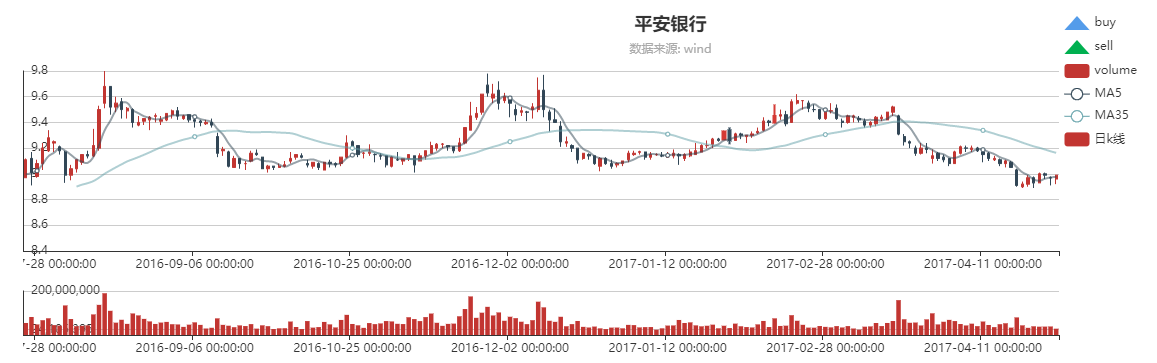
\includegraphics[scale=0.5]{figures/ma_exp.png}
	\caption[移动平均线示例]{移动平均线示例}
	\label{fig:maexp}
\end{figure}

从上文可以看出,技术分析指标种类繁多,不同类型的指标可能适用于不同的标的物(例如:指数、蓝筹股、小盘股)。老练的技术分析者完全可能通过对不同股价走势的同时观察,由此产生多个技术指标信号成为交易决策的依据,从而实现对多个股票的市场数据挖掘。

除了以上琳琅满目的技术指标外,技术分析专家还可以通过观察蜡烛图的形态和颜色,找到一些形态类的特征。例如:M头、W底、圆弧底、头肩底、红三兵、三只乌鸦、仙人指路等等。形态类利用的数据实质上是OLHC蜡烛图数据。形态类的特征还有波浪理论,波浪理论通过对之前行情的“波浪”进行计数,以判断当前牛市(或熊市)的绝对位置。均线或平滑异同移动平均线(MACD)等的技术指标也可绘制成副指标图,形成了多头排列、空头排列、金叉、死叉等被技术分析派认为反映了市场多空力量对比的特征。

技术分析者研究得出的技术分析特征具有一定价值,陈等在2019年引入了MACD、RSI等传统技术分析形成的特征\cite{chenfangfang2019},再使用随机森林(random forest)和boosting等方法执行了预测任务,最终获得了较好的效果。需要注意,仅是特征提取并不能完整地囊括技术分析的所有流程。

提取了特征后,老练的技术分析交易者会根据自己的经验和见闻来对特征进行取舍。以上所列的一系列技术分析特征,最终只被保留很少的部分,作为技术分析者使用的交易系统的基石。需要注意,简单的交易系统往往是特定市场环境下,经过技术分析玩家长期的市场实践,优胜劣汰留下的系统,其涵义与研究者随机抽取的交易系统存在区别。因为,长期市场的优胜劣汰实则为交易系统的演进提供了温床。简单使用这些特征并不能反应技术分析交易系统的全貌。

本文虽然没有使用技术分析作为特征提取的传统的PV因子择时模式,但这种市场数据挖掘模式在金融研究和量化投资领域是被给予了相当的重视的,因此,在此简略介绍。

\section{技术分析与参数优化}

技术分析在真实市场中的表现形态复杂多样,真实市场中,优秀的$f$、$\theta$将是一个可盈利的交易算法的核心。在此,可将真实市场中的技术交易系统的步骤进行如下总结,本文将根据以下简化了的技术分析交易系统构建策略:
\begin{itemize}
	\item 由技术分析系统盯市,并产生交易信号
	\item 产生信号后,对信号进行过滤或二次确认
	\item 接入买入算法交易模块
	\item 接入卖出策略、风险控制等模块
\end{itemize}
产生这样一个技术分析交易系统,往往是经过市场数据回测检验和实盘检验,并不断进行参数的调整和优化,最终,将形成一个被老练技术分析交易者所使用的稳定的技术分析框架。因此,技术分析系统的参数具有动态性。本文将把$\theta$视为可学习的,而学习目前就是上式中的得分函数最优化,也就是,将信息比率最优化。

为何要使用这样一种参数优化的方式来解释技术分析交易系统呢?因为,市场人士普遍认为,技术分析如果能够盈利,那么,其盈利的关键要素一定不是指标或系统,而是运用技术分析的交易者以及随之配套的“神奇参数”。例如,有一种基于技术分析的交易方法被称之为炒单。炒单的意思是,交易者完全凭借自己脑海中复杂的神经网络系统,根据市场上盘口数据的信号,直接依赖直觉捕捉交易机会,以博取差价。技术高超的炒单员可能积少成多、聚沙成塔,达到稳定盈利的目标。\\
\begin{figure}
	\centering
	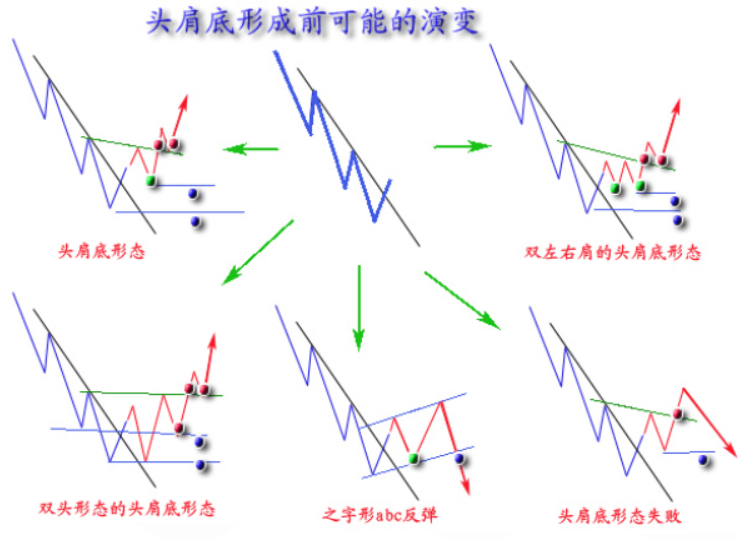
\includegraphics[width=0.7\linewidth]{figures/ta-1.png}
	\caption{金融标的价格走势的底部形态\footnote{图片来源于新浪博客 http://blog.sina.com.cn/u/6013942202}}
	\label{fig:ta-1}
\end{figure}
基于价格走势图形的直觉式下单,或称炒单,则是市场数据挖掘的一种极端的形式。这个极端的形式对于$s_{t-1}$的挖掘直接通过人脑的极端复杂的超大规模的神经网络来进行。这个超大规模的生物神经网络的权重和参数是由交易员累积的经验所习得的,与本文在机器学习的视角下,对技术分析体系进行参数优化的方法颇有类似。对于直觉式下单,或称“炒单”,目前没有足够的研究材料。但对于高频交易的下单问题,人工交易也是大型量化投资机构的选项。

Bojinov等在2017年分析了某大型量化投资机构的人工交易与算法交易的优劣,该文章构造了随机化的时间序列实验方法以及因果估计目标(causal estimand),据此对比了人工交易与算法交易的金融滑点(slippage)的优劣\cite{Iavor2019Time}。该研究的结果是,某些任务中,人工交易滑点更低,而某些任务则相反。从市场的角度来理解,人工下单的执行力和反应速度都是不及算法的,但人类的直觉式下单可以在复杂环境下对当前局面进行直觉性的判断,也具备迅速举一反三的小样本学习能力,这是算法难以做到的。因此,在算法交易所考验的低市场冲击、隐藏交易信息等方向,人类的直觉也并非一无是处。

从机器学习的角度来看,技术分析的指标或形态,仅仅能提供一个分析框架,机器学习模型最终的预测效果,有赖于数据驱动(data-driven)产生的训练后的权重。

在机器学习的框架下,如果我们有$N$个训练样本:$\{(x_1,y_1),...,(x_N,y_N)\}$。这里,$x_i$是第$i$个样本的训练样本,而$ y_i $则是第$ i $个目标(target)。机器学习此时需要寻找一个函数$ g(x) $,使得$ g(x)=\arg\min_y \mathcal{L}(x,y) $。其中,$ \mathcal{L} $是损失函数,一般是函数$g$的拟合优度。

\begin{equation}
R_{emp}(g)=\frac{1}{N}\sum_i \mathcal{L} (y_i, g(x_i))
\end{equation}

如何定义损失函数$\mathcal{L}$,以及,如何寻找$g$,就是机器学习所关心的问题。对于这个问题,最常见的解决方法是经验风险最小化(empirical risk minimization)或称为损失函数最小化(loss minimization)\cite{Vapnik2000The}。上式就是经验风险的表达式。经验风险最小化通常会使得函数$g$最优地切合训练数据。但如果函数$g$过于注重切合训练数据,往往就会造成对于新数据的预测能力的下降。这在机器学习领域被称为过拟合(overfitting)。对此,统计学家采用结构化的风险最小化(structure risk minimization)来寻找$g$,具体来说,结构化风险在确定$\mathcal{L}$上做文章,常常会引入惩罚项(panalty)来控制预测方差,提升模型的泛化能力,或称模型上线后的表现。有关泛化能力的定义如下式:
\begin{equation}
R_{online}(g)=\frac{1}{M}\sum_i \mathcal{L}(y_i, g(x_i)),
\end{equation}
其中,$M$是新数据的个数。最终,机器学习的学习目标是产生具有优秀泛化能力的模型,泛化能力好的机器学习模型具有以下两个特点:
\begin{itemize}
	\item $ R_{emp}(g) $足够小;
	\item $R_{online}(g)$与$ R_{emp}(g) $的差距足够小;
\end{itemize}

同样,如果不引入市场数据对技术分析交易系统进行优化,那么,技术分析就相当于一个未经训练的神经网络或随机森林的模型,自然不具备认为预测市场的能力,也就不具备盈利能力。因此,本文提出机器学习技术分析(machine learning technical analysis)的方法,通过优化回测结果来调整参数。这将在很大程度上模拟交易员对技术分析交易系统的打磨和调参,正如,机器学习专家对机器学习的有关模型进行训练一样。只有被市场数据训练过的技术分析模型才能被认为是贴近于市场交易真实情况的技术分析交易模型。

\section{参数优化的实现}
在机器学习领域,系数或权重(weights)(类比于本文技术分析体系中的参数)的优化方式有多种。经典线性模型中,满足一定条件下,权重的最优解存在闭式解(close-formed)。对于岭回归而言,我们也可以通过矩阵运算,高效地求出解析解。岭回归是防止线性回归出现过拟合,降低泛化误差的一种有效手段,它实际上是引入了inductive bias来帮助算法更为正确的理解实际情况。

对于以下损失函数的优化:
\begin{equation}
||Ax-b||_2^2 + ||\Gamma x||_2^2
\end{equation}
其中,$x$是可变的系数,Tikhonov矩阵$\Gamma$是经过合理选择的。此Tikhonov回归存在显式解,写作$\hat{x}$,

\begin{equation}
\hat{x}=(A^{T}A+\Gamma^{T}\Gamma)^{-1}A^{T}b.
\end{equation}

但是,复杂的机器学习算法中,让损失函数最小化的权重往往是不存在显式解(explicit solution)的。甚至,损失函数本身可能也不是凸(convex)的,或者是不光滑(smooth)的,这意味着可能存在多个局部最优解。对于反向传播神经网络(BP neural network),常见的优化方法是基于反向传播的梯度下降(gradient descent)算法。

梯度下降算法有很多变体,机器学习领域,基于一阶梯度的算法有:随机梯度下降(Stochastic Gradient Descent)、动量(momentum)、Nesterov加速算法、Adam、AdaGradient等等。这些算法中,Adam是实际效果最好的\cite{Kingma2014Adam}\cite{Nesterov2017Efficiency}。统计机器学习领域,最小角回归算法(least angle regression)也是一种梯度下降算法\cite{Tibshirani2004Least},实际上,LAR算法是让系数朝着拥有最大梯度的坐标方向移动,而当存在两个梯度一样的方向时,先动某一个方向则意味着下一次会移动另一个方向,如果学习率趋近于0,则最终会形成系数坐标沿着角平分线路径运动的效果。

梯度下降为基础的优化算法(gradient based method)是当今机器学习领域几乎仅存的优化策略,但本文所研究的技术分析交易系统,其损失函数$\mathcal{L}$需要通过回测求得,梯度更是无从谈起。因此,我们需要通过其他的方法对技术分析交易体系的参数进行优化。

而自Fama\cite{Malkiel1970EFFICIENT}从上世纪中叶开展有效市场理论的研究以来,大多数研究对于技术分析的设定和定义都是参数静态的。而对参数的调整也是技术分析交易系统的一部分,甚至,参数的调整和确认可能是比交易系统本身更为重要的一部分。不调整参数的技术分析交易模型,就像是未经精调(fine-tuning)的深度学习模型,其效果不能代表技术分析的真正实力。

前文提到,人类的直觉在交易领域依旧占据一席之地。同理,也可以通过模拟人类直觉调参的方式来对技术分析交易系统进行优化。如同围棋游戏,人类通过棋感和围棋知识来缩小搜索范围,技术分析参数的确定,也可以理解为和alphago\cite{Silver2017Mastering}类似的缩小状态空间(state space)的搜索范围的问题。因此,本文将顺着这个思路,一步一步解决机器学习的参数优化问题。

下面,我先来构建一个朴素的双均线交叉的做多策略:
\begin{enumerate}
	\item 定义 $MA_{k,t}=(1/m_k)\sum_{i=t-m_{k-1}}^{t-1}p_i $,其中,$k=1,2,3,4$;
	\item 定义 $y_1\%, y_2\%$;
	\item 买入信号:$MA_{1,t-1}>MA_{2,t-1}$;
	\item 买入信号确认:$MA_1$和$MA_2$呈上升趋势,其$t-1$时刻的一阶差分大于等于0;
	\item 过滤信号:$MA_{3,t-1}>MA_{4,t-1}$;
	\item 产生买入信号后,如果信号得到了确认,且经过了过滤,则全仓买入;
	\item 退出策略:当股价上升$y_1\%$后,盈利退出;当股价下降$y_2\%$后,止损退出。
\end{enumerate}

对以上交易算法,我们需要调整6个参数,分别是$m_1,m_2,m_3,m_4,y_1,y_2$,通过对这6个参数的调整,使得定义的经验得分$\mathbf{Score}$最大化。其中,$\theta=(m_1,m_2,m_3,m_4,y_1,y_2)$,而$\Theta$是参数空间,代表所有可能的$\theta$取值。一般来说,技术分析体系下,第一条均线被称为快线,代表短期趋势。第二条均线是慢线,代表中期趋势。而过滤信号中的两条均线中,其中一条往往是代表长期趋势或牛熊状态的超慢线。同时,止盈率$y_1\%$和止损率$y_2\%$也有一定的取值范围,一般短期策略的止盈率和止损率都降低,长期策略的止盈率和止损率较高。具体的$\Theta$取值将在本章下一节详细介绍。

与机器学习的各类算法不同的地方在于,得分函数是不可导的,并且每次求得分函数都需要经过回测(backtest),而回测的计算成本很大。对于以上参数优化,最显而易见地是可以通过穷举法(brute-force method)来进行搜索,如此可以找到对应参数空间内的全局最优解。

对于连续值参数,全局穷举常常被简化为栅格点搜索(grid search)。栅格点搜索的具体方法是,对于$\Theta$中的所有取值的可能进行了离散化,形成了一系列的格点。本文中,$\Theta$实则是一个高维的多面体,通过对这个多面体内部的离散化的一个个的格点进行遍历,我们就能找到所期待的参数组合。

栅格点搜索的优势在于,它可以找到接近全局最优的解(如果栅格点的划分够细的话),但由于这个算法需要遍历离散化后所有可能的参数组合的取值,因此,计算开销十分巨大。以本文所提出技术分析策略系统而言,这样的计算开销是难以承受的。由于栅格点搜索的开销过大,机器学习任务中常见的参数选择方法还有随机搜索(random search)。

随机搜索牺牲了全局最优,使得参数优化得到的解的质量呈现出更大的风险。随机搜索假设参数服从某种易于抽样(sampling)的概率分布。最简单的随机搜索可以假设参数服从独立的均匀分布,算法将从这个多维分布中不断抽样,达到终止条件后,选择效果最好的参数组合。

以下是随机搜索的参数优化算法\cite{Hastie2004The}。
\begin{enumerate}
	\item 设定所有参数的联合分布$\Pr(\theta|\beta)$(实际应用中,也可假设参数之间相互独立);
	\item 设定迭代次数N;
	\item 进行N次循环,每次都从联合分布中抽取一个参数组合$\theta$;
	\item 从以上产生的参数组合中,选择能让损失函数$\mathcal{L}$最小化的参数组合;
\end{enumerate}

随机参数搜索的运行速度和效率远远高于栅格化搜索,但由于随机噪声的缘故,其准确性相对较差。

模拟量子退火(simulated annealing)也是一种随机搜索。该算法产生的第一个解是随机生成的,此后,产生的新解由旧解加上随机扰动而产生。产生新解后,算法会判断新解对于目标函数是否有改进。如果有改进,则接受新解,否则,算法将以可变概率拒绝新解,这个概率随着迭代次数的增加而增加。模拟退火算法具有渐进收敛性,已在理论上被证明以概收敛于全局最优解\cite{Hwang1988Simulated}。

那么,现实生活中,老练的技术分析交易者是如何确定技术分析交易系统的参数的呢?答案很可能是直觉。这就像围棋专业九段的棋感一样,老练的技术分析交易者能以少量的迭代步骤找到一个适用于市场的技术分析系统参数。这个过程类似于贝叶斯优化(bayesian optimization)\cite{Pelikan2005Bayesian}。贝叶斯优化常用于损失评估成本较高时的机器学习的调参任务,例如,大型神经网络调参。大型神经网络的训练需要大量的gpu时,成本十分巨大。此时,贝叶斯优化称为了一个有力的工具。贝叶斯优化是当前机器学习、深度学习、数据挖掘领域中,应用最为广泛的超参数(hyper parameter)优化手段。

对技术分析系统进行回测同样是相当耗费算力的,尤其是对于大量时间序列进行事件驱动(event driven)的模拟交易性质的回测。同时,贝叶斯优化于老练的技术分析交易员的调参手段也颇具类似性,老练的技术分析玩家的调参过程与基于序列模型的优化(Sequential model-based optimization,SMBO)有异曲同工之妙,有关SMBO的内容我将在下一小节详细介绍。

人工智能首次战胜职业棋手的算法alphago\cite{2016Mastering}使用了蒙特卡洛树搜索和深度卷积神经网络。Alphago Fan采用了两个神经网络,一个负责评估策略空间,另一个负责评估。因此,这两个网络又被称为策略网络和价值网络。其中,策略网络$p_\sigma$是基于监督学习的,学习的材料是人类的棋谱。对于任何一个局面(state),该策略网络可以返回作为人类,下一步棋可能落子的位置。alphago算法在此基础上进行计算和推演,再运用价值网络进行判断,最终找到算法所认为的最有利于获胜的招法。


真正市场中的技术分析交易系统的参数选择,往往也依赖于技术分析的老手对盘面数据、回测数据的观察,之后采取的跳跃式的、类似神经网络的预测。SMBO算法中的核心是对不同参数组合产生的损失进行预判$p(y|x)$。同时,制定获得函数(acquisition function)主动获得新的参数组合与损失的对应的数据,以进一步将之前的预判准确化。

此处,预判$p(y|x)$类似于一种直觉,以及alphago通过监督学习所训练得到的棋感。而获得函数$S$则需要平衡探索(exploration)和局部优化(exploitation),是基于直觉的一种策略,类似于经验丰富的操盘手调整参数以试探市场获得更多的信息。贝叶斯优化的流程是,从一个参数的实例出发,通过模型来判断可能的结果优秀的下一个参数实例。随后,进行成本较高的结果判断得出$(x_i,y_i)$,再将其整合进数据集$\mathcal{D}$根据新的信息,修正以往的判断模型。再从当前的参数实例出发,寻找下一个可能结果优秀的参数实例,以此类推。

SMBO算法是贝叶斯优化的基本形式,这个算法的核心是找到一个模型,通常是基于统计机器学习的,使得我们可以根据以往的结果来预判可能的结果优秀的参数。目前,常见的模型可以是高斯过程(Gaussian process)甚至可能是随机森林(random forest)或神经网络(feed-forward neural network)。
而技术分析参数的形成也是如此。经验丰富的技术分析者,一开始会使用市场上流传的默认参数,随着时间的推进,他们会观察市场的情况,以此来训练大脑中的真正的生物神经网络。再运用这个神经网络来寻找下一个可能的结果优秀的参数。本文也将通过贝叶斯优化来还原老练的技术分析者调校、打磨其交易系统的过程,并检验最终的决策系统的盈利性。

\section{基于贝叶斯优化的技术分析交易体系}
本文所测试的技术分析交易体系,其参数将是可变的,其中,优化参数的方法基于栅格点搜索、随机搜索和贝叶斯优化。根据上一节中列举的双均线交易算法,我们需调整6个参数,分别是$m_1,m_2,m_3,m_4,y_1,y_2$。分别代表移动平均线的快线周期、慢线周期、用于确认的移动平均线的快线周期和慢线周期,以及止盈比例和止损比例。

\subsection{基于高斯过程的贝叶斯优化}
贝叶斯优化\cite{Pelikan2005Bayesian}是栅格点搜索、随机搜索以及人工调参的良好替代,其特点是能够在探索(exploration)和最大化利用(exploitation)之间取得均衡。在机器学习领域,贝叶斯优化(bayesian optimization)可被用来优化各种各样的损失函数的交叉验证值,或称交叉验证损失(cv loss),交叉验证损失被认为是泛化误差的一个比较准确的代理\cite{Arlot2009A}。在机器学习领域,损失函数的选择是多样的,可以是基于负对数似然(negative log-likelihood)、精确性(accuracy)或F1得分。本文将从更广义的角度思考问题,所选择的得分函数$\mathcal{L}$为之前定义的信息比率。

对此,我们需要对求出下列问题的解:
\begin{equation}
x_{opt}=\arg\max_{x\in\mathcal{X}}\mathcal{L}(x),
\end{equation}
此处,方程$\mathcal{L}:\mathcal{X}\rightarrow\mathbb{R}$是一个运算成本很高的函数,这里指交易回测;$\mathcal{X}\subset \mathbb{R}^d$是一个欧式空间内的有界的矩形(box),结合之前的技术分析交易体系$d=6$。贝叶斯优化在实践中被证明适合对随机的、非凸等复杂情况的函数进行优化,且与经验丰富的技术分析交易员人工调参可以类比。以下是基于序列模型的优化(Sequential model-based optimization,SMBO)的具体过程。


\begin{enumerate}
	\item 输入:$\mathcal{L},\mathcal{X}, S, \mathcal{M}$;
	\item 初始抽样:$\mathcal{D}\longleftarrow \mathbf{INIT SAMPLES}(f,\mathcal{X})$
	\item 以下迭代指标从$|\mathcal{D}|$到总样本数循环;
	\item 训练模型$M, \mathcal{D}$,产生$p(y|x,\mathcal{D})$;
	\item 根据获得函数得到$x_i$的值:$x_i=\arg\max_{x\in\mathcal{X}} S(x, p(y|x, \mathcal{D})$;
	\item 得到新数据(这一步成本较高):$y_i=\mathcal{L}(x_i)$, 并将其整合进$\mathcal{D}$;
	\item 重复4-6直到迭代终止。
\end{enumerate}

以上算法中,$\mathcal{L}$就是之前定义的得分函数——信息比率。其定义为:
\[
\mathcal{L}=\mathbf{IR}=\frac{r}{\sigma_r},
\]
其中,$\bar{r}$是对应的策略的年化收益率,$\sigma_r$为年化标准差。在实际处理的过程中,股价经过了复权处理,并以人民币计价,最终的计算过程如下:
\[
\bar{r}=(1/T)\sum_{i=1}^{T}(\log{p_{i+1}}-\log{p_{i}})\cdot(250/T),
\]
\[
\hat{\sigma_r} = \sqrt{\frac{1}{T-1}\sum_{i=1}^{T}(\log{p_{i+1}}-\log{p_{i}}-\bar{r}\cdot T/250)^2\cdot\sqrt{250/T}},
\]
上式中的$p_i$为一定初始资金条件下,在$i$时刻的净值。要求得得分函数$\mathcal{L}$需要将策略进行模拟交易,得到净值曲线pnl(profit and lost)再依据净值曲线求得信息比率。

本文仅使用信息比率这一最经典的指标来对策略进行评价,投资者也可使用其他风险、收益指标来充当得分函数。

SMBO算法中的$\mathcal{X}$在本文中是一个$d$维的欧式空间中的多面体,但实际上也可以是其他形状,它代表了各个参数的可能的取值域笛卡尔积。$S$指代的是获得函数(acuisition function),这个函数在贝叶斯优化中负责控制探索(exploration)和最大化利用(exploitation)之间的平衡。获得函数由$\mathcal{M}$计算而得,通常是易于优化的一个函数。求得获得函数的最大值的$x$常常是在$\mathcal{X}$中,兼具探索性和利用价值的点,在这个点计算成本较大的得分函数是值得的。

获得函数的有多种选择方式,常见的有
\begin{itemize}
    \item 高斯过程上置信界(Gassian Process-Upper Confidence Bound,GP-UCB):
    \[
    x_t=\arg\max_{x\in\mathcal{X}}\alpha_t(x)=\arg\max_{x\in\mathcal{X}}\mu_{t-1}(x)+\beta^{1/2}\sigma_{t-1}(x).
    \]
    该获得函数所求最小值的部分,实质上,基于高斯过程的SMBO算法是对$\{x_i\}$建模后求得的后验分布的均值和后验标准差的加权和。其中,$\mu$项是基于已确定的模型的,因此,代表对已有模型的最大化利用(exploitation);$\sigma$项代表对已有模型可能的不确定性的推断,最大化这一项代表对可能产生最优解区域的探索,因此,这一项代表对未知的探索(exploration)。
    \item 期望提升(expected improvement, EI):
    \begin{align*}
    x_t &= \arg\max_{x\in\mathcal{X}}\mathbb{E}_{f(x)\~\mathcal{N}(\mu_{t-1}(x),\sigma^2_{t-1}(x))}[\max(f(x)-f^{+}_{t-1},0)]\\
    &= \arg \max_{x\in\mathcal{X}}(\mu_{t-1}(x)-f^{+}_{t-1})\Theta(\frac{\mu_{t-1}(x)-f_{t-1}^+}{\sigma_{t-1}(x)})+\sigma_{t-1}(x)\phi(\frac{\mu_{t-1}(x)-f_{t-1}^+}{\sigma_{t-1}(x)}),
        \end{align*}
    此处,$\Theta$和$\phi$分别表示标准一元高斯分布的概率密度函数(pdf)和累计分布函数(cdf)。这个式子只考虑提升的可能,在计算期望的时候,过滤掉了导致降低表现的可能,因之被称为期望提升函数。EI的实用性极强,很多实现贝叶斯的软件包使用了EI作为获得函数。
    \item 基于信息论的获得函数\cite{Hoffman2014Predictive}:
    \[
    x_t =\arg\max_{x\in\mathcal{X}}\mathbb{H}\left[p(x_*|\mathcal{D})\right]-\mathbb{E}_{p(y|\mathcal{D}_n,x)}\left[\mathbb{H}[p(x_*|\mathcal{D}_n\cup\{(x,y)\})]\right],
    \]
    此处H表示信息熵,代表信息量或不确定性。该获得函数能获得最大信息量的新样本$x^*$进行高成本的损失函数计算。但实际运算中,由需要对以上获得函数进行近似计算。
\end{itemize}

以上列举了几种可用的贝叶斯优化的获得函数。除了获得函数的不同外,SMBO算法中的回归模型$\mathcal{M}$的也可有差异。目前开放的一些软件包多使用EI(expected improvement)作为获得函数,而回归模型又有多种,例如,高斯过程(Gaussian process)、树结构的Parzen估计(tree Parzen estimation)和随机森林(random forest)\cite{shahriari2015taking}。

本文在使用高斯过程作为SMBO的建模方法,使用高斯过程上置信区间作为获得函数,其原因是,这样的算法组合适用于本文的参数空间。之后的实证结果表明,使用基于高斯过程的贝叶斯优化能够很好地在训练集上找到显著盈利的交易策略。

%---------------- Chapter 4 ---------------------------


\chapter{实证分析}
股票市场是随着时间推移而不断发展、变化的市场,股票市场的效率常常也随着时间的推移而不断提高。根据之前的综述,对于中国股市是否达到了有效性这点,学术界存在着一定争议。某些研究认为中国股市没有达到弱有效,某些研究则认为技术分析或其他市场数据挖掘方法能产生超额的收益。

本文将在重点探讨2017年与2018年两年期间的股市有效性,具体来说,是中证500指数的所有成分股的走势,是否符合有效市场假说。我国股市经历了多轮牛熊更替,也经历了诸多重大国际国内金融事件的洗礼,截止到本文定稿,中国股市是否已经达到了弱有效,这将是一个有待发掘的问题。同样,技术分析作为一种国内散户投资者和部分机构投资者都相当青睐的投资手段,其在这些股票上的盈利能力,也需要实验来检验。此外,广大散户投资者投入了大量的时间和精力在技术分析上,如果技术分析并不能从市场中赚钱,那么,他们宝贵的时间和精力就没有必要花费在技术分析上了。

\section{数据来源与准备}
本文将研究2017年及2018年两个年份的中证500指数成分股的日线级别的蜡烛图(candle chart)数据。中证500指数的股票样本选择了那些A股“普通”市值不太大的


从多个角度探索仅凭历史价格数据能否挖掘出盈利模式的问题,进而回答中国股市是否达到弱有效?以下是本文数据概况。
\begin{table}[H]
	\centering
	
\begin{tabular}{|c|c|}
	\hline
	类型 & 说明 \\
	\hline
	数据时间 &  2017年~2018年;\\
	\hline
	数据内容 &  股票代码、日期、OHLC数据、涨跌幅、成交量、成交额\\
	\hline
	数据来源 & tushare金融数据平台\cite{tushare} \\
	\hline
	数据大小 &  153.7MB\\
	\hline
	样本数量 & 100000+\\
	\hline
	时间序列条数 &  1000+条\\
	\hline
	周期类型 & 日线级别\\
	\hline
\end{tabular}
\caption{本文所使用的数据}
\end{table}



对于OHLC数据,本文并全部使用,本文所使用的特征为涨跌幅、收盘价。本文数据库保障了平均每条时间序列含有约694个时间周期,因此,双均线策略中被认为威力较大的百日线或150日均线也可以被良好计算。之后本文会进行类似机器学习的训练测试分离(training test split)处理,即便如此,平均每条时间序列也可保证350个时间周期。不过在之后的处理过程中,部分时间周期数量不足的股票因为无法适用双均线交易系统而被舍弃。本文包含ST和*ST股,因为他们也是中国股票市场的一部分。

本文的数据获取方式是通过tushare api来提。tushare金融数据接口是一个免费、开源的python财经数据接口,可实现对股票市场数据及基本面数据的数据采集。本文通过该api采集的数据,返回pandas数据框\cite{mckinney2012python}。本文采用csv文件存储这些数据,如果数据量更大,也可使用mongodb或mysql数据库进行处理。

本文采用的数据经过tushare专门的接口进行了前复权处理。因为真实市场中的股价是经过除权(dividend exclusion)的,因此,我们需要对股票价格进行复权。复权处理又分为前复权和后复权,前复权的意思是将历史股价进行复权处理,但保持现价不变,其优点是稳定,缺点对于过于久远的历史数据可能存在精度问题(因除权计算的四舍五入)。后复权则是保持历史价不变。考虑到本文分析周期等因素,本文采用的是前复权。


\subsection{本文假设}



本文的核心研究对象为股票市场的价格行为,故进行假设:投资者可以按照每日收盘价进行买卖,并不需考虑市场流动性的深度和广度。此处也不考虑滑点(financial slippage)。

这条假设对于大多数股票都是成立的,即便是涨跌停的个股,也常常拥有一些买入和卖出的机会,但仍有部分股票难以在涨停和跌停价格买入或卖出。不过,涨跌停制度实际上也是股票交易制度的一部分,如果涨跌停制度在某种程度上影响了股票价格的有效性,那么,这种有效性的损失也是包含在本文研究范畴内的。

本文主要研究股票市场的价格行为,因此,未剔除ST股(亏损股)或*ST股以及新股,因为这些都是市场的组成部分。

\subsection{实验准备:回测框架}
本文采用向量化的方式回测,因此,回测(backtest)速度比较快。python社区的数据分析模块pandas\cite{hilpisch2014python}和numpy都支持向量化运算,可避免循环枚举,大幅提高了回测速度,使得本文在较小的计算资源条件下(单核Xeon Processors @2.3G)也可完成大规模的回测和处理。之后进行的随机化实验也利用了pandas的良好性能。当然,如果面对更大的数据(big data),则有更适合的方法。

使用pandas框架中的rolling和聚合函数方法,以及pandas自带的时间处理模块,均可对本文所涉数据进行合理地处理,并计算出我需要的技术分析信号。需要注意,我们需要使用shift方法来将时间线左移一位,以确保每个时间点所产生的技术分析信号都是来自于历史数据的。如果没有进行shift,则会使用未来函数,使得分析结果出现偏差。

本文的核心研究对象为股票市场的价格行为,故进行假设:投资者可以在当天利用收盘价进行研究,并于第二天开盘,以开盘价买进。考虑到散户投资者的资金容量并不大,因此,本文没有考虑市场流动性的深度和广度及由此产生的市场冲击成本问题。由于中国股市运行地是集合竞价制度,此处也不考虑滑点(financial slippage)。这条假设对于大多数股票都是成立的,即便是开盘涨跌停的个股,也常常会有一些买入和卖出的机会,当然,有部分股票难以在涨停和跌停价格买入或卖出。不过,涨跌停制度实际上也是股票交易制度的一部分,如果涨跌停制度在某种程度上影响了股票价格的有效性,那么,这种有效性的损失也是包含在本文研究范畴内的。



\section{Wald-Wolfowitz游程数检验}
在使用回测框架进行测试之前,我们2017年的数据进行游程数检验。Wald-Wolfowitz游程数检验也可简称游程检验(runs test),是一种检测二值序列随机性的假设检验方法,它可以检测序列的相互独立性(mutually independent)。一个游程(run)就是元素完全相同的最大的序列区段,举例来说:

AAAABBBAAAAABBBBAAAAA
含有以下游程“AAAA”、“BBB”、“AAAAA”、“BBBB”和“AAAAA”,因此,以上序列含有的游程数为5。

游程检验的零假设为:
\begin{itemize}
    \item 零假设:对于一个二值序列,其每个元素都抽样来自独立的相同的分布。
\end{itemize}

在零假设下,游程数(runs)基于A与B的个数($N_A,N_B$)的条件分布可以被认为是近似正态的,其两个参数,均值和方差为:
\begin{itemize}
    \item 均值$\hat{\mu}=\frac{2N_A N_B}{N}+1$
    \item 方差$\hat{\sigma}^2=\frac{(\mu-1)(\mu-2)}{N-1}$.
\end{itemize}
上式中,N为总的元素个数。根据以上条件可以构造正态统计量。
\[
\mathcal{Z}=\frac{R-\hat{\mu}}{\hat{\sigma}},
\]
在零假设下,该统计量近似标准正态分布。那么,如果这个统计量高于或低于某个阈值,则可认为序列非随机,各个元素之间相互独立的假设就应该被拒绝。

\subsection{实验结果}

本文将游程检验应用于股票市场有效性检验之中,选取2017年到2019年三年的深圳市场所有股票的行情数据进行分析。对于其中某一条时间序列,我们持有面板数据,将面板数据中的pct\_chg字段进行处理,如果这个值大于0,则标记为“+”,否则标记为“-”。
经过以上处理,对每个股票而言,都会形成一条由“+”和“-”两个值构成的二值序列,再对这个二值序列进行游程检验,即可得到对应的结论。表5-2呈现了部分实验结果。
% Please add the following required packages to your document preamble:
% \usepackage{graphicx}
\begin{table}[]
\centering
\begin{tabular}{cccc}
\hline
No.  & Code      & Z         & p\_value \\ \hline
973  & 002524.SZ & -0.035505 & 0.971677 \\
2056 & 300669.SZ & 0.601846  & 0.547277 \\
1420 & 300021.SZ & 0.568125  & 0.569950 \\
1455 & 300057.SZ & -0.155860 & 0.876144 \\
1254 & 002818.SZ & 2.747613  & 0.006003 \\
1511 & 300115.SZ & 1.866397  & 0.061986 \\
1232 & 002793.SZ & 0.671066  & 0.502179 \\
2105 & 300720.SZ & 0.959330  & 0.337393 \\
138  & 000552.SZ & 2.699816  & 0.006938 \\
814  & 002364.SZ & 1.411554  & 0.158081 \\ \hline
\end{tabular}
\caption{游程检验部分实验结果}
\end{table}

表中数据以均匀抽样的方式,从深圳市场全体个股的数据中,抽取了10只个股的游程检验数据。其中有两只股票被拒绝,这两只股票的走势不符合游走(random walk)假设。

再举例进一步分析,代码为002818.SZ的股票,其游程检验p值为0.006。实际上,该股属于2016年年末上市的新股,上市期间出现了大幅上涨的情况,随后,17到19年则呈现出单边下跌的走势,从此角度分析,A股市场一直未能对该股准确估价。其中一部分原因是涨跌停制度,另一部分原因可能是市场本身不够有效。

对于深圳市场整体的2195只股票而言,游程检验p值小于0.05的股票个数为348只,占比为15.85\%。(表5-3)

根据以上内容以及图5-1,我们可以认为深圳市场中有15\%的股票不符合随机游走,而有85\%的股票通过了游程检验,呈现出弱有效性。未通过检测的比例较以往的研究有所下降。游程检验在一定程度上可以得到有关股票市场有效性的结论,但对于广大投资者来说,这个检验得出了有超过15\%的股票是非有效的,且并不能直观地回答技术分析能不能赚钱这个问题。

因此,本文将进一步通过数据挖掘的手段,论文中国股市是否达到了弱有效性。


\begin{table}[]
\centering
\begin{tabular}{lll}
\hline
Num\_reject & Num\_all & Percentage \\\hline
348         & 2195              & 0.1585 \\\hline
\end{tabular}
\caption{游程检验对于2196只个股的结果}
\end{table}

\begin{figure}
    \centering
    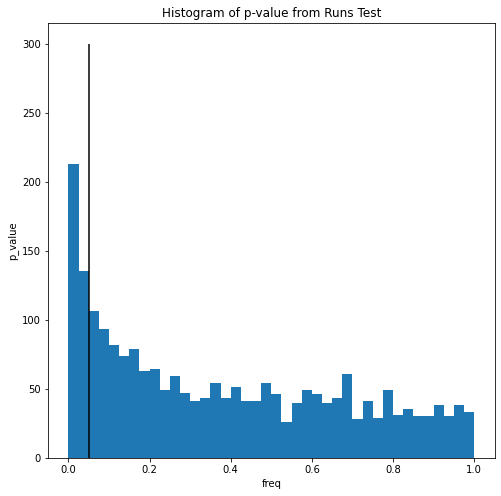
\includegraphics[scale=0.7]{fig5-1.png}
    \caption{游程检验p值分布直方图}
    \label{fig:my_label}
\end{figure}


\section{贝叶斯优化技术分析:以收益率为目标}

本文所使用的技术分析交易系统需要优化5个参数,分别为$ma_1$、$ma_2$、$fma_1$、$fma_2$,其取值范围分别为0到30、31到60、61到100、101到200。从优化的角度来看,除了前文提到的类似经验丰富的技术分析专家调参的贝叶斯优化方法外,机器学习领域常用的优化算法还有栅格点搜索(grid search)或随机搜索(random search),此外还有多种模拟动物行为或物理现象的优化算法。本节将阐述贝叶斯优化相较栅格点搜索以及随机搜索的优势。

\subsection{对比:贝叶斯优化对比栅格点搜索及随机搜索}
下面简述栅格点搜索的算法:
\begin{enumerate}
    \item 让$ma_1$从1到30之间枚举
    \item 让$ma_2$从31到60之间枚举
    \item 让$fma_1$从61到100之间枚举
    \item 让$fma_2$从101到200之间枚举
    \item 进行回测,计算损失函数(或得分),保留最好的结果
    \item 重复以上步骤直到枚举完毕
\end{enumerate}

栅格点搜索(grid search)不适用于本文的实验,因为其计算过程很缓慢。经过实验,计算机无法在2个小时内产生程序结果。因为数据量庞大,进行一次回测所需时间约为1.03(0.01)秒。经过计算,栅格点搜索需要运行的时间为7416000秒,约合2060小时。如果对随机抽样的500只股票施展栅格点搜索,时间还需要翻500倍。

从理论上来说,栅格点搜索可以获得全局最优解(global optimization),但其运行时间是无法接受的。

接下来,我来对比贝叶斯优化与随机搜索,随机搜索(random search)的基本步骤为:
\begin{enumerate}
    \item 让$ma_1$从1到30之间等可能抽样
    \item 让$ma_2$从31到60之间等可能抽样
    \item 让$fma_1$从61到100之间等可能抽样
    \item 让$fma_2$从101到200之间等可能抽样
    \item 进行回测,计算损失函数(或得分),保留最好的结果
    \item 重复以上步骤直到达到迭代次数完毕
\end{enumerate}

对比贝叶斯优化,随机搜索没有进行exploitation和exploration的权衡。因此,其效果从理论上来说应该是不如贝叶斯优化的。

本文所使用的贝叶斯优化算法在上一章理论环节已经进行了详尽阐述。本文采用高斯过程(Gaussian Process)作为概率建模工具,同时使用上置信界(Upper Confidence Bound,UCB)作为获得函数。这一套贝叶斯优化的实现方案是目前实现最广的方案。

以000001.SZ股票为例,表5-4说明了随机搜索优化进行30轮迭代的过程及效果。贝叶斯优化的得分为0.534,而随机搜索优化的得分为0.367,可以说贝叶斯优化的效果要明显优于随机搜索优化,其运行的时间也在可接受的范围内。
\begin{table}[h]
\centering
\begin{tabular}{ccc}
\hline
iterations & BO    & Random Search \\\hline
30         & 0.534 & 0.367        \\\hline
\end{tabular}
\caption{30次迭代后随机优化与贝叶斯优化得分效果对比(结果为收益率得分,下同)}
\label{tab:my-table}
\end{table}


\begin{figure}[h]
    \centering
    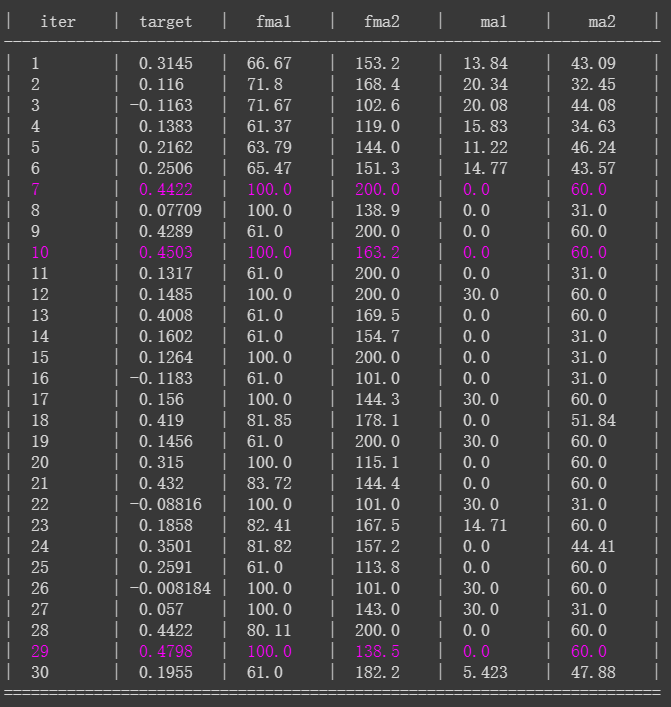
\includegraphics[scale=0.9]{fig5-2.png}
    \caption{贝叶斯优化的迭代过程示例}
    \label{fig:my_label}
\end{figure}

\subsection{贝叶斯优化轮次确定及其与买入并持有策略效果的对比}
图5-2提供了一个贝叶斯优化进行迭代的过程的示例,为了在较为经济的计算量下,获得有说服力的结论,本文首先需确定合理的迭代轮次,因此,我进行了以下工作:
\begin{itemize}
    \item 从所有股票数据中,随机抽取100只股票作为样本;
    \item 对这100只股票及技术分析交易系统分别执行10轮、20轮及30轮贝叶斯优化,并观察其效果;
    \item 抽取500只股票作为样本;
    \item 根据第2步的结果,选择最为经济有效的轮次,再对500只股票用这样的轮次进行贝叶斯优化,得最终结果。
\end{itemize}

表5-5展示了对随机抽取的100只股票,进行不同轮次的贝叶斯优化所拿到的得分。可以看到,20轮迭代的结果明显高于10轮迭代的结果,而30轮迭代的结果较20轮迭代的结果的提升是有限的。


\begin{table}[h]
\centering
\begin{tabular}{ccc}
\hline
iterations & BO    & Buy and Hold \\\hline
10 & 0.1779& -0.2970\\
20 & 0.2335& -0.3082\\
30         & 0.2437 & -0.2885        \\\hline
\end{tabular}
\caption{不同轮次贝叶斯优化得分对比同有效交易周期的买入并持有策略}
\label{tab:my-table}
\end{table}

因此,考虑到计算成本问题,本文随机抽取500只股票作为样本后,将采用20轮迭代的贝叶斯优化,来对技术分析双均线交易系统进行参数优化。下表将展现500只股票中随机抽取的10只个股,其经过20轮贝叶斯优化了的技术分析交易系统的交易得分与买入并持有策略对比的结果。

\begin{table}[h]
\centering
\begin{tabular}{cccc}
\hline
    & \textbf{code} & \textbf{BO} & \textbf{BuyAndHold} \\ \hline
180 & 000921.SZ     & 0.415294    & -0.330302           \\
408 & 000702.SZ     & 0.168606    & -0.936058           \\
436 & 002381.SZ     & 0.200257    & -0.033111           \\
353 & 300208.SZ     & 0.167344    & -0.994378           \\
170 & 300022.SZ     & 0.115285    & -0.376527           \\
447 & 000929.SZ     & 0.248791    & -0.741236           \\
299 & 002149.SZ     & 0.067850    & -0.511152           \\
63  & 000050.SZ     & 0.186652    & -0.282015           \\
242 & 001965.SZ     & 0.101715    & -0.069424           \\
36  & 002191.SZ     & 0.416220    & 0.159378            \\ \hline
\end{tabular}
\caption{随机抽取的10只股票贝叶斯技术分析与买入持有策略比较}
\label{tab:my-table}
\end{table}

\begin{figure}[h]
    \centering
    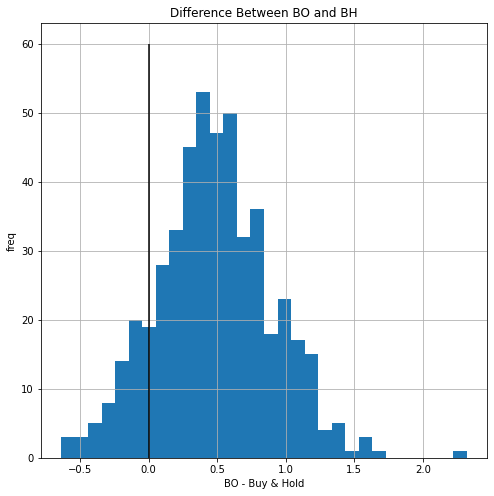
\includegraphics[scale=0.7]{fig5-3.png}
    \caption{贝叶斯优化技术分析策略与买入并持有策略的差异图}
    \label{fig:my_label}
\end{figure}
数据表明,对于87\%以上的股票而言,贝叶斯优化可以提升技术分析交易系统的市场数据挖掘能力,使得这些交易系统的得分提升(或使得损失降低)。贝叶斯优化无法使得对应的技术分析交易系统取得更好效果的股票之中,买入并持有的收益率较高,均值为0.5430,远远高于500只样本的均值-0.235。

\subsection{贝叶斯技术分析系统随机化测试}
贝叶斯优化能不能有效从市场中挖掘信息?对于这点,上一小节已将贝叶斯技术分析同随机交易进行了对比。本节将从随机化实验出发,探讨经过了贝叶斯优化技术分析系统是否能显著地强于随机交易,如果它可以显著地强于随机交易,则可以认为,贝叶斯技术分析作为一套择时系统,具备一定市场数据挖掘能力。

本节将展开两项实验,首先是比较单个个股,贝叶斯优化技术分析、未经调参的技术分析与随机交易的优劣;第二是500只股票作为股票池平均持有作为资金管理则略的前提下,比较贝叶斯优化技术分析与随机交易的优劣。

\section{蒙特卡洛随机化实验设计}
本文考察技术分析的择时能力,因此,采用蒙特卡洛打乱检验(Monte Carlo permutation tests)的方式是非常方便的\cite{dwass1957modified}。该检验的检验统计量的计算方法是依照零假设生成的所有可能的值组成的。如果标签是可交换的,那么对应的检验可获得精确显著性水平,随之可计算置信区间。

\subsection{个股的贝叶斯技术分析与随机交易的对比}
本节为选择了一只个股,代码为000004.SZ,股票名称为“国农科技”,来探讨对这个股票走势施展贝叶斯优化技术分析交易与随机交易的差异。为此,我构建了一个假设检验:
\begin{itemize}
    \item 零假设$H_0$:贝叶斯优化技术分析交易与随机交易无差异
\end{itemize}

对于随机交易,我采取以下方式构建:
\begin{enumerate}
    \item 确立周期数$T$以及每日涨跌幅$d_1,...,d_T$;
    \item 先从等可能有限格点分布$\{1,2,...,T\}$中,抽取一个数$t$,作为总持股长度;
    \item 在从${1,2,...T}$中无放回地均匀抽取$t$个样本,作为随机交易的持股期
\end{enumerate}
在$H_0$满足的条件下,根据Glivenko-Cantelli定理,不断进行随机抽样的情况下,经验分布以概率1收敛于潜在的分布,因此,在样本数量足够的前提下,我们可以用随机交易产生经验分布,再以此来比较贝叶斯优化技术分析与随机交易的优劣。实验结果如图5-4,计算得p值为0.006。
\begin{figure}[h]
    \centering
    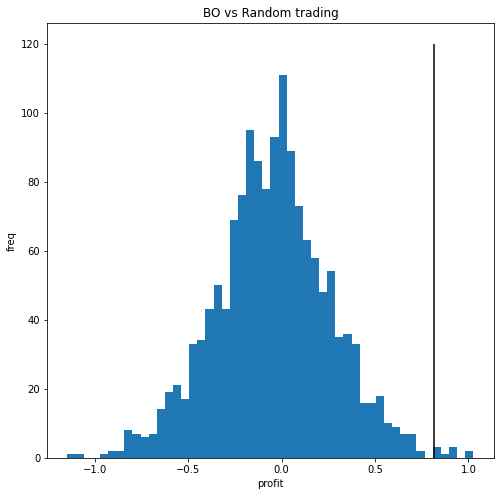
\includegraphics[scale=0.7]{fig5-4.png}
    \caption{贝叶斯优化技术分析(黑线)与随机交易的比较}
    \label{fig:my_label}
\end{figure}

以上结果表明,对于个股而言,贝叶斯优化技术分析可以展现出强大的市场数据挖掘能力,贝叶斯优化可在一定程度上释放技术分析交易系统的能力和潜力。下图5-5是未经调参的技术分析交易系统(双均线系统)与随机交易作比较,依据下图很难断言,未经调参的技术分析交易系统要优于随机交易。


\begin{figure}[h]
    \centering
    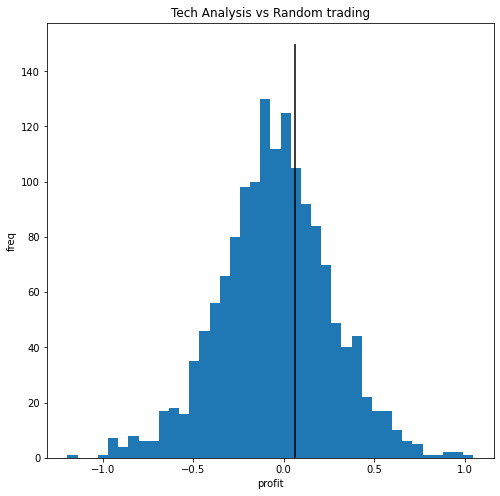
\includegraphics[scale=0.7]{fig5-5.png}
    \caption{无优化技术分析(黑线)与随机交易的比较}
    \label{fig:my_label}
\end{figure}


\subsection{多股贝叶斯技术分析与随机交易的比较}
本节抽取了500只股票,由于双均线策略周期计算等原因,剔除了其中16只不满足条件的股票,将其余484只股票视为一个整体,考察贝叶斯优化技术分析能否优于随机交易。为此,本节暗含了一个基于个股平均分配的资金管理策略。

该资金管理策略假设投资者将资金平均分配给484只股票,因此,最终的收益率为每只股票收益率的简单平均数。在随机交易方面,每只股票产生一个随机持有序列及收益率,最终将484只股票的收益率予以平均,则得到随机交易的一个收益率实例,如此重复,则可得出随机交易收益率的经验分布。

本实验的零假设与上一小节无异,但本节贝叶斯优化技术分析交易及随机交易的内涵按上一段来操作,与上一小节不同。

\begin{itemize}
    \item 零假设$H_0$:贝叶斯优化技术分析交易与随机交易无差异
\end{itemize}

对个股而言,随机交易也是通过以下方式构建:
\begin{enumerate}
    \item 确立周期数$T$以及每日涨跌幅$d_1,...,d_T$;
    \item 先从等可能有限格点分布$\{1,2,...,T\}$中,抽取一个数$t$,作为总持股长度;
    \item 在从${1,2,...T}$中无放回地均匀抽取$t$个样本,作为随机交易的持股期;
\end{enumerate}

\begin{figure}[h]
    \centering
    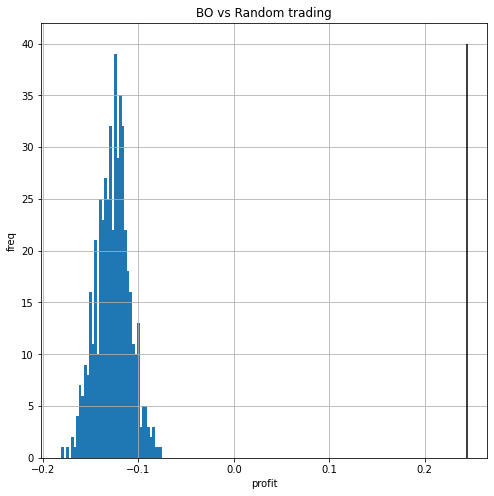
\includegraphics[scale=0.7]{fig5-6.png}
    \caption{贝叶斯优化技术分析对比随机交易2}
    \label{fig:my_label}
\end{figure}

根据图5-6,贝叶斯优化技术分析的得分显著高于随机交易(p=0.000)。

\subsection{本小节总结}
本小节及之前的内容,从各个角度论证了贝叶斯优化加持的技术分析交易体系的强大的市场数据挖掘能力。

本文之所以使用技术分析及贝叶斯优化来进行市场数据挖掘,一方面是因为,这样的组合接近于广大投资者笃信的技术分析,另一方面,这样的组合自由度较低,可有效防止过拟合。

但,以上研究并不能证明或证伪股票市场的弱有效性,仅仅展现了贝叶斯技术分析的市场数据挖掘能力。这说明了,如果市场有一定技术分析相关的规律,那么技术分析是可以将其挖出来的。以往的一些研究往往将未经参数调整的技术分析,或仅是数个参数组合格点的技术分析作为技术分析的代表,对比本文方法,则说服力较弱。

下节,我将引入机器学习的模型评价方法,最终将判定中国股市是否达到了弱有效,以及技术分析到底能不能从股票市场中赚钱。

\section{深圳市场弱有效性的测试}
经过之前的研究和论证,贝叶斯优化技术分析具备良好的市场数据挖掘能力。同时,其模仿有经验的技术分析交易者的调参过程,搭配传统技术分析体系,可以说较贴切地模拟了市场上的技术分析交易手法。

那么,这样的交易手法能否从市场中赚钱?这需要从机器学习的角度来论证。机器学习将数据集分为训练集和测试集,其中,训练集又可做k折交叉验证(k-fold cross validation)。这就是机器学习领域常见的训练-测试流程。本文所采用的流程在之前的理论章节已有详尽描述,此处则主要谈执行层面的问题。

\subsection{测试集500只个股的贝叶斯优化效果}

本小节将整个数据集中trade date予以划分,按照日期的中位数为界限,之前的数据划分为训练集,之后的数据划分为测试集。实验流程与之前类似,但这次是对训练集进行贝叶斯优化后,再由测试集来测试结果。

需要说明,因为将时间序列对半切分,因此,又有一定数量的时间序列因为周期数量达不到双均线策略的要求而被舍弃。

以下是初步测试结果:

\begin{table}[h]
\centering
\begin{tabular}{ccc}
\hline
iterations & BO    & Buy and Hold \\\hline
10 & 0.0595& 0.063515        \\\hline
\end{tabular}
\caption{贝叶斯优化技术分析效果(新数据)}
\label{tab:my-table}
\end{table}

从这个收益率得分的均值来看,贝叶斯优化从已观测数据(observed data)中挖掘了大量信息,产生了相当高的盈利,但其在新数据(unseen data)中表现一般。图5-7的随机化实验的结果也说明了这一点。

\begin{figure}[h]
    \centering
    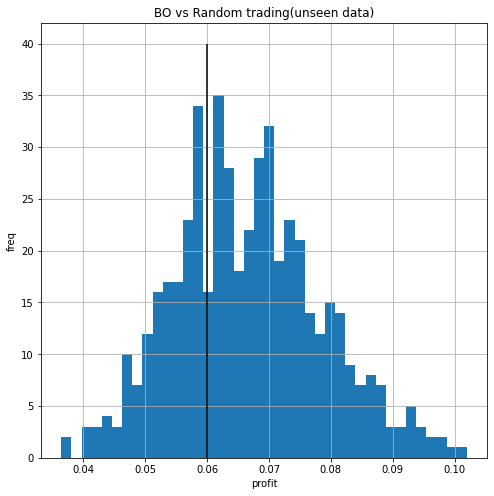
\includegraphics[scale=0.7]{fig5-7.png}
    \caption{贝叶斯优化技术分析(黑线)对比随机交易(新数据集)}
    \label{fig:my_label}
\end{figure}

从以上实验中可以得出结果,贝叶斯优化技术挖掘可以挖掘出已知市场数据的盈利空间,但到了测试集中,其效果却与随机买卖相近。

\subsection{抽取20只个股,是否存在赚钱机会?}
从整体市场而言,对于新数据(unseen data)贝叶斯优化技术分析无法显著优于随机交易,那么,对于个股而言,是否存在赚钱机会呢?

本小节同样使用了之前采用的随机实验,不过,实验对象是从2196只股票中,随机抽取的20只个股。实验结果如下图5-8所示。

\subsection{小结}
前几个小节通过大量实验展现出贝叶斯优化技术分析拥有良好的市场数据挖掘能力,其盈利得分可以显著优于随机交易。

但面对新数据,之前挖掘出来的模式(pattern)或盈利系统,则不再能够盈利。总体的盈利水平与随机交易无显著差异。

\begin{figure}[h]
    \centering
    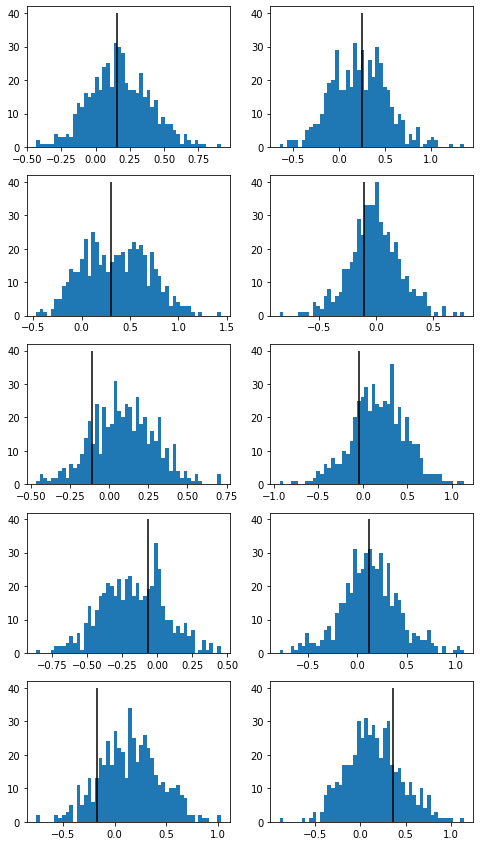
\includegraphics[scale=0.7]{fig5-8.png}
    \caption{20只个股贝叶斯优化技术分析对比随机交易(新数据)}
    \label{fig:my_label}
\end{figure}




%------------------------Chapter----------------
\chapter{结论}
本文通过构建机器学习技术分析并运用贝叶斯优化对基于市场信息的技术分析交易系统予以建模,机器学习技术分析这个概念将传统的股票市场技术分析与机器学习结合了起来,并使用贝叶斯优化模拟了老练的交易员的交易系统。

本文将运用这套市场数据挖掘系统对深圳市场的所有股票数据进行了挖掘,在训练期(formation period)内,贝叶斯数据挖掘系统能够有效地挖掘出股票市场的盈利模式,获得可观的择时收益,并且显著由于随机择时。相较于以往的研究,这证明了贝叶斯优化可以将市场中的盈利模式挖掘出来。

但依照机器学习技术分析,训练期获得显著的盈利仅能证明该系统可以从市场数据中“学习”到盈利模式。金融市场是否存在可供利用的错误定价,中国股市是否在日线、双均线系统下达到了弱有效,这取决于交易期能够获得利润。实验证明,之前挖掘出来的盈利系统在面对新数据时不再能盈利了,总体盈利水平与随机交易无显著差异。

这最终说明:股票市场纷繁复杂,瞬息万变,双均线系统所挖掘出来的“规律”不具备时间稳定性,因此,相关策略难以在深圳市场中盈利。进一步可以推断,基于日线市场数据分析的传统的技术分析极有可能丧失了盈利空间。广大投资者不应在技术面分析上浪费太多时间。本文的实验也进一步支撑了深圳市场已经达到弱有效性的结论。





%附录部分
\appendix

%自动生成参考文献列表,需要模板根目录下有:bib/thesis.bib
\bibliographystyle{lzubib}
\bibliography{bib/thesis}


%致谢
\begin{thanks}
Ajouter de la vie aux jours lorsqu'on ne peut plus ajouter de jours
à la vie.

\end{thanks}


\end{document}
